\documentclass{article}
\usepackage{graphicx}
\usepackage{hyperref}
\usepackage{imakeidx}
\usepackage{rotating}
\usepackage{multirow}
\usepackage{array}
\usepackage[export]{adjustbox}
\usepackage{geometry}
\setcounter{secnumdepth}{4}
	
\usepackage{pdflscape}

\title{Trama Principale}
\author{Giovanni Cisternini}
\makeindex

\begin{document}
\tableofcontents

\maketitle

\section{Introduzione personaggi}
    \subsection{Intro Nadar e Vidar}
    Approdano al porto di Neverwinter dopo l’ennesima scorribanda, scendono e respirano a pieni polmoni. Conoscono abbastanza bene Neverwinter, ci sono stati un po' di volte principalmente per bere alla locanda del Leviatano Spiaggiato, non sono esattamente clienti abituali, ma sanno come funziona il posto, ma dato che sono appena le 9 del mattino decidono di seguire la strada che si erano prefissati ed arrivare a questa gilda di Avendwarfs per vedere cosa vogliono …
    \subsection{Intro Thia}
    Arriva dalla porta nord-est di Neverwinter, ci è già stato altre volte principalmente per acquistare merci e trovare informazioni, sa di essere nel Quartiere delle Torri, ma non sa benissimo dov’è la casa per cui chiede in giro e ci arriva facilmente …
   
    \subsection{Intro Bryseis}
    Arriva dalla porta sud-est, appena entra si sente a casa, conosce molto bene Neverwinter, sa che posto meraviglioso può essere, ma soprattutto non sente la pressione degli occhi che la fissano e la giudicano …
    Intro Atalanta e Cassiopea: mancano per poco Bryseis, ma entrambe si incontrano per puro caso alla porta Sud- Est… si salutano festosamente… ma nessuna delle due è mai stata a Neverwinter per cui non sanno dove andare
    \subsection{Intro Atalanta e Cassiopea} mancano per poco Bryseis, ma entrambe si incontrano per puro caso alla porta Sud- Est… si salutano festosamente… ma nessuna delle due è mai stata a Neverwinter per cui non sanno dove andare
\section{PNGGilda}
\subsection{Dexter}
Mezzorco secco e bassino un po' spelacchiato con un accento strano che fa da portinaio e lavora a maglia ( ha fatto pace con Nadarr)
\subsection{Sugar}
Nano con pancia che fa da cuoco
\subsection{Johnny}
Mezzelfo con i capelli bianchi e i baffi bianchi che fa da tutto fare
\subsection{Thorgrim}
Thorgrim, discendente dei nani delle montagne, nato circa a metà di uno dei periodi più bui per Faraun, si trova già in tenera età immischiato con la compagnia dell'Ascia Insaguinata, di cui facevano parte i suoi genitori. Dopo circa 160 anni conosce all'interno di questa, un paio di umani, un barbaro, Rollo Moon, e una cantastorie, Ambreide Silver , con cui instaura un rapporto tra l'amicizia e il partenale. I due ebbero 2 figli, uno di sangue, Wulfric, e una adottiva, una mezzelfa, Sylas, a cui Thorgrim fini per fare da Nonno adottivo e da Mentore dopo la dipartita dei genitori. Thorgrim, è molto gioviale e gentile nei modi, pur nascondeno un lato che brama il potere e la forza, difatti è sempre stato temuto sia dai suoi rivali che compagni per  la sua ferocia e aggressività in battaglia. Molto rigido quando si tratta di sgominare gli avversarsi, pur essendo infondo un animo gentile per quanto riguarda i bambini. Non ha mai apprezzato ne condiviso la crudelta dei suoi compagni ed è per questo che circa 2 anni prima degli eventi attuali ha fondato assieme a Wulfri e Sylas una compagnia di ventura  che puntasse si al compimento di missioni e battaglie ma anche alla salvaguardia del popolo. Nano corpulento con braccia spesse e muscolose, con l'avanzare dell'età è apparsa una bella pancia da birra, ha segni di battaglia ovunque sul corpo e sul viso, una lunga barba brizzolata, che copre appena una cicatrice sul labbro, capelli scuri con vari ciuffi bianchi. Porta con se sempre il suo Guanto Bianco da paladino, la sua pipa da casa e una cintura con strumenti da carpantiere, nel suo ufficio sono appesi le sue armi e armature, indossa sempre una canotta bianca con sopra un gilett che si chiude a stento e dei pantaloni tenuti su da una cintura in pelle.
\subsection{Wulfric}
Wulfric, figlio di sangue  di Rollo Moon e Ambreide Silver, cresce forte e coraggioso come il padre, con un carattere mite e simpatico nei momenti di calma, e aggressivo e feroce in battaglia, sotto la guida del nonno e mentroe Thorgrim, riesce a controllare gli istinti animaleschi della Licantropia ereditati dal padre. Si guadagna il soprannome  Bloody all'età di 26 anni durante una battaglia, svolta al chiaro di luna piena, in cui perde il controllo poiché feriscono gravemente la sorella minore, Sylas,  e diventa una bestia simil lupo che squarta i suoi nemici con ferocia e brama di sangue, al termine della battaglia non ricorda nulla e gli viene raccontato da suo nonno Thorgrim, quella era la seconda volta che perdeva il controllo in quel modo, la prima fu all'età di 12 anni, quando scopri di aver perso i suoi genitori per colpa di un traditore dell'ascia insaguinata. In preda all'ira omicida, diede la caccia al drow traditore e lo squarto. Thorgrim riusci ad insegnargli come controllare i suoi istinti e quindi riuscire ad accettarsi e controllare i suoi poteri. Ama sua sorella più di ogni altra cosa e fa di tutto per proteggerla. Wulfrick è un bestione di 1,96, molto robusto e muscoloso, indossa un gile con pelliccia, e ha una cicatrice sull'occhio sinistro, occhi chiari e capelli corvini, barba nera e folta, e ha il simbolo degli avendwarfs sul braccio sinistro, come tutti i bestioni è un po' tonto per cui non apprende subito segnali e altro, bisogna essere molto chiari con lui. Il suo istinto animale non gli procura solo aggressività ma anche una gran fame che accompagna con litri di birra. 
\subsection{Sylas}Sylas, sorella adottiva di Wulfric, non conosce i suoi veri genitori, sa solo che Rollo e Ambreide l'hanno trovata quando aveva appena 1 anno e che l'hanno accudita come se fosse loro figlia dal primo momento, per questo non ha mai avuto intenzione di cercare i suoi genitori biologici e ne gli interessava più di tanto, anche perché era stata ulteriormente adottata da Nonno-Thorgrim. Sylas, fin da piccola ha sempre adorato cantare e suonare, e l'Ascia Insanguinata era il posto perfetto per far pratica poiché composti da molte persone, che si erano spietati assassini e malfattori, ma non disgnevano certo la musica e fra loro c'erano molti Bardi da cui imparare arti di vario genere, dalla musica, alla danza, alla seduzione, crescendo diventa una mezzelfa molto bella e avvenente, con forme normali e una voce melodiosa e stupenda, occhi verdi e molto grandi, capelli castani e un sorriso molto dolce, sul 1.75. Ha un carattere molto estroverso quando deve intrattenere e fare amicizia, ma tende ad essere molto chiusa quando deve parlare di se in determinati argomenti. È gentile ed altruista, molto furba , ma con poco senso del pericolo, motivo per cui è sempre sgridata da Wulfric, che la protegge sempre. Si è guadagnata il suo soppranome durante il periodo in cui lavorava come mercenario, intrattenendo i compagni durante le notti fredde con storie e canzoni, utilizzando il flauto di pan, fatto in argento, della madre che le ha insengnato molto. 
\subsection{Artella}
Artella, gnomo delle rocce, fuggita dal suo piccolo villaggio in cerca di avventura e conoscenza, fin da piccola ha una passione sfrenata per la tecnologia e la magia, tant'è che impara a fodere le 2 cose e creare oggetti con funzionalità più disparate. Scappa via all'età di 17 anni, e incontra thorgrim e i suoi nipoti nei pressi di Waterdeep mentre stava cercando di fabbricare una spada che fosse in grado anche di sputare fuoco, fallendo. Gnoma alquanto robusta e muscolosa per la sua statura, indossa sempre degli occhiali da saldatore e una tunica da fabbro regalatogli dal padre  all'età di 12 anni . Pur essendo molto piccola, è molto aggressiva e peperina, non ha paura di affrontare nessuno, nemmeno Wulfric, infatti spesso lo sfida a duello per testare le sue nuove invenzioni, odia essere accarezzata la testa e solitamente da una martellata sul piede a chi ci prova. Il suo martello è particolare perché è in grado di ingrandirsi in caso di combattimento e rimpicciolirsi quando deve lavorare. 
\subsection{Pippa} Pippa Astuta, nata all'incirca nel 1459, scappata dalla sua terra , Mulhorand, all'età di 12 anni perché schiava, figlia di contadini era stata catturata da un gruppo di banditi che avevano distrutto il suo villaggio, venduta poi sul mercato nero come moglie-bambina, riusci a scappare dal suo padrone dopo circa 2 anni di abusi e torture. Ha sulla  schiena cicatrici di frustate e il tatuaggio degli Avendwrafs che copre il marchio impresso dal suo ex padrone Atlhestan, e dei tatuaggi lungo i polsi che rapresentano delle corde . All'età di 15 anni riesce a lasciare la sua terra, ed iniziare il viaggio verso l'ignoto, viaggia molte e fa esperienze di ogni tipo. All'età di 25 anni incontra Thorgrim e i suoi nipoti durante un'esplorazione nei pressi di Waterdeep. Thorgrim riesce in qualche modo a conquistare la fiducia di Pippa Astuta, la quale dato il suo passato aveva perso ogni tipo di stima nei confronti di ogni umanoide. Decide di unirsi e di aiutare Thorgrim e i nipoti nella loro missione.
\section{PG}
\subsection{Penelope}Penelope nata a Hillsfar, fin da piccola stringe una forte amicizia con un bambino poco più grande di lei di nome Simon. I due si sposeranno e avranno tre bambini Etan, willie e Anton.
Penelope vive felicemente con la sua famiglia per 15 anni. Una sera però, mentre penelope non era in casa, tutta la sua famiglia muore in un incendio. Vedendo tutti i suoi concittadini disinteressarsi dell’incendio lei inizia a provare un profondo odio verso di loro a tal punto da diventare un accolito della dea Shar(Dea della Perdita) .


\subsubsection*{Habitants di Hillsfar}

\paragraph*{Descrizione di Hillsfar}
Hillsfar è una pittoresca città commerciale situata sulle colline verdi della regione di Arvandor. Le sue strade tortuose sono piene di vita, con il mercato centrale che vibra di attività mentre i cittadini fanno affari o chiacchierano tra loro. Le torri dei maghi e le botteghe degli artigiani si ergono al di sopra dei tetti, creando un profilo urbano unico contro il cielo azzurro.

\paragraph{}*{Negozi di Hillsfar}

\begin{itemize}
  \item \textbf{La Bottega di Agata} - Un negozio di erboristeria gestito dalla gentile Agata, che vende una vasta gamma di erbe e pozioni curative.
  \item \textbf{La Fucina di Brannor} - Un'officina di un fabbro tenuta dal muscoloso Brannor, dove si possono trovare armi e armature di ottima qualità.
  \item \textbf{La Locanda del Drago Fumante} - Un'accogliente locanda gestita da Edric, che serve piatti abbondanti e birra della casa.
  \item \textbf{La Galleria d'Arte di Elara} - Uno spazio artistico tenuto dalla talentuosa Elara, dove si possono acquistare dipinti e sculture uniche.
\end{itemize}

\paragraph*{Cittadini di Hillsfar}

\begin{enumerate}
  \item \textbf{Nome:} Alan Stone\\
  \textbf{Famiglia:} Stone\\
  \textbf{Professione:} Fabbro presso La Fucina di Brannor

  \item \textbf{Nome:} Penelope Greenleaf\\
  \textbf{Famiglia:} Greenleaf\\
  \textbf{Professione:} Proprietaria de La Galleria d'Arte di Elara

  \item \textbf{Nome:} Harold Smith\\
  \textbf{Famiglia:} Smith\\
  \textbf{Professione:} Contadino

  \item \textbf{Nome:} Rebecca Blackwood\\
  \textbf{Famiglia:} Blackwood\\
  \textbf{Professione:} Cuoca presso La Locanda del Drago Fumante

  \item \textbf{Nome:} Thomas Rivers\\
  \textbf{Famiglia:} Rivers\\
  \textbf{Professione:} Bibliotecario presso La Biblioteca di Hillsfar

  \item \textbf{Nome:} Lily Willow\\
  \textbf{Famiglia:} Willow\\
  \textbf{Professione:} Fioraia

  \item \textbf{Nome:} Marcus Strong\\
  \textbf{Famiglia:} Strong\\
  \textbf{Professione:} Guardia cittadina

  \item \textbf{Nome:} Sophia Gold\\
  \textbf{Famiglia:} Gold\\
  \textbf{Professione:} Sarta
\end{enumerate}




\subsection{Bryseis}Molti sono i pregiudizi legati a noi teifling, per il legame con il principe dell’inferno Asmodeo, e questo non fa altro che generare odio su di noi. Quando ero molto piccola, un gruppo di soldati e maghi umani spaventati dal nostro aspetto demoniaco ha attaccato il mio piccolo villaggio nonostante fosse pacifico da generazioni. Durante l’attacco i miei genitori sono stati uccisi ma io, nonostante fossi stata gravemente ferita sulla schiena (cosa di cui ancora oggi porto la cicatrice), mi sono salvata rifugiandomi nella foresta vicina. La rabbia e il dolore dell’accaduto hanno risvegliato in me la magia assopita da generazioni e con un fulmine a ciel sereno si è palesata davanti ai miei occhi una piccola pallina di luce che mi ha tenuto compagnia in quella bruttissima notte, solo il giorno dopo però ho capito che ero diventata uno stregone. Da quel momento io e gli altri bambini sopravvissuti abbiamo deciso di vivere insieme ai limiti più degradati di una città molto popolosa e piena di nobili. Io sono diventata una criminale al fine di racimolare i soldi per riuscire a sopravvivere e a sfamare anche gli orfani più piccoli di cui mi prendevo cura come una sorella maggiore. Passavo quindi le mie giornate a borseggiare i nobili e a cercare di duplicare i guadagni a poker, gioco in cui nel tempo sono diventata molto brava. Quando anche i piccoli sono cresciuti abbiamo deciso di prendere strade diverse per lasciare i bassifondi e puntare tutti ad una vita migliore. A tal fine ho cominciato a viaggiare per il mondo cercando una nuova famiglia in una gilda e ponendomi due obiettivi di vita: far cambiare idea e abbattere i pregiudizi che ci sono sui teifling e vendicare i miei genitori cacciando e uccidendo il manipolo di uomini che ha ucciso la mia famiglia. 
\subsubsection{Rete di Criminali}
\subparagraph{Sindri Timbers aka Il Fantasma}
È un gracile ma atletico gnomo delle foreste alto poco più di 60 centimetri con gli occhi grigi ma i capelli nerissimi, che fanno risaltare la sua pelle estremamente chiara. Più grande di me di 2 anni, quindi attualmente ha 27 anni. Ci siamo incontrati da bambini, quando avevamo 10 e 12 anni, qualche mese dopo la morte dei miei genitori. Prima di arrivare nella città dove io e i bambini superstiti del mio villaggio ci siamo poi stabiliti, viaggiavamo per le foreste vagando alla cieca alla ricerca di una nuova casa. Una notte ci fu una tempesta bruttissima con fulmini, saette e pioggia torrenziale e, per non rimarci secchi, io e gli altri bambini ci siamo rifugiati in una grotta. Dentro la grotta abbiamo incontrato un minuscolo gnomo addormentato e tremante, così piccolo che per poco uno dei piccoli dragonidi non gli spappolava la testa con un piede. Disturbato dal nostro arrivo e dal piede di Vortex a due millimetri dal suo naso, lo gnomo si è svegliato ma invece di prendersela per averlo quasi ammazzato, in men che non si dica si è tirato su con un salto e ha cominciato a saltellare e roteare per la caverna con un’agilità e un’eleganza degna di un ballerino, il tutto senza mai smettere di parlare alternando domande del tipo “e tu chi sei?” a piccoli racconti della sua vita e battute dal dubbio gusto. Alla fine, esasperata, l’ho afferrato con la mia coda e solo allora siamo riusciti a comunicare come si deve. Abbiamo così scoperto il suo nome e cosa ci faceva lì: Sindri era scappato dalla sua casa che si trovava nel fitto di quella stessa foresta per inseguire il sogno di diventare il più grande gioielliere del mondo, dimostrando a tutti che nonostante fosse così piccolo (il più piccolo del suo villaggio e per questo preso poco seriamente da tutti) poteva riuscire in qualsiasi cosa volesse. Dato che entrambi eravamo in cerca di una città dove stabilirci abbiamo ripreso il nostro viaggio insieme diventando così amici. Arrivati in città abbiamo cominciato a derubare i ricchi insieme non solo per sfamarci ma anche per recuperare i materiali che gli sarebbero serviti per esercitarsi a forgiare i suoi gioielli. Quando è riuscita a completarla, mi ha regalato la sua prima creazione ufficiale: un piccolo orecchino d’oro, rotondo con una piccolissima gemmina di ossidiana incastonata all’interno, che tutt’ora ho indosso. Sindri era il perfetto partener in crime: la sua agilità, la sua furbizia e il suo orecchio fino ci hanno salvati milioni di volte dall’essere arrestati, o peggio. Queste stesse caratteristiche sono state notate da un gruppo di scaltri criminali specializzato nel reperimento e la divulgazione d’informazioni di qualsiasi genere, i “Moonlight Cipher”, che lo ha invitato ad entrare nella loro rete. Nonostante non volesse accettare l’invito, per via del suo sogno di fare il gioielliere, ad oggi Sindri è uno dei membri più bravi, con diversi sottoposti. In particolare, è specializzato nel trovare il modo di recapitare messaggi senza essere visto non solo dal ricevente ma anche dal mittente del messaggio (ecco per “il fantasma”) e nel recuperare informazioni dai luoghi più segreti del pianeta. Quando ci siamo separati, l’una per andare ad esplorare il mondo in cerca di una nuova famiglia e l’altro per entrare nei Moonlight Cipher, abbiamo trovato il modo di rimanere sempre in contatto fra di noi. Il giorno che se n’è andato mi ha lasciato un bigliettino e un fine braccialetto dorato con al centro incastonata una strana pietra rossa (dello stesso colore della mia pelle). Il bigliettino spiegava come usarlo. In ogni luogo di ritrovo di criminali e manigoldi, di qualsiasi città del mondo, nascosto da un’illusione agli occhi di tutti tranne che a chi fosse abituato, come me, a vedere oltre le sue illusioni, lui avrebbe fatto in modo di disegnare uno speciale simbolo magico. Avvicinato il braccialetto al simbolo quest’ultimo avrebbe reagito prendendo in prestito una briciolina del mio potere del fulmine per inviare un’innocua scossa all’identico braccialetto che Sindri porta al polso. La scossa avverte Sindri della mia convocazione e in men che non si dica, grazie alla sua schiera di aiutanti e alla rete di criminali di cui fa parte, riesce a scoprire dove mi trovo e a presentarsi per darmi una mano. 
\subsection{Nadarr}Nadarr lama d'ottone, era il secondo di tre fratelli Dragonici. Vive la sua infanzia e, parte dell'adolescenza, insieme ai suoi fratelli tra le stradine strette di una piccola città portuale. Raggiunti i 14 anni (12 umani) decide di imbarcarsi in una nave mercantile per esplorare il mondo ma soprattutto vivere il mare, contro il volere di suo fratello maggiore. Durante una delle traversate il mercantile viene attaccato da una nave pirata, qui viene arruolato da Vidar con cui stringe un forte legame di fratellanza BROOOOO. E diventa, a tutti gli effetti, un pirata.  Negli anni successivi, tra un'azione piratesca e l'altra incontra, in uno dei tanti porti visitati, un orchessa Cassiopea con cui ha un breve relazione. I due però di separano per via delle loro vite complicate e vagabonde.
\subsection{Vidar}Nel cuore delle terre selvagge di Faerûn, in un piccolo villaggio vicino alle Montagne Spine del Mare, nacque Vidar. Figlio di un'umana e di un mezz'orco, Vidar crebbe in una comunità che spesso guardava con sospetto la sua straordinaria mescolanza di sangue. Fin dalla giovane età, il suo aspetto imponente e la sua forza sovrumana attirarono l'attenzione, ma anche l'isolamento. Vidar, tuttavia, era dotato di un'anima ribelle e un cuore avventuroso. A 16 anni, stanco delle restrizioni del suo villaggio, decise di intraprendere una strada diversa. Sentiva il richiamo del mare e la chiamata delle avventure che lo aspettavano al di là dell'orizzonte. Il giovane mezz'orco sognava di solcare i mari, di diventare un pirata temuto e rispettato. Abbandonando la sua casa dietro di sé, Vidar si diresse verso la costa, armato solo della sua fedele ascia e della determinazione di forgiare il proprio destino. Giunto al porto, si imbarcò su una nave mercantile, desideroso di imparare le arti della navigazione e della vita marina. Durante il viaggio, Vidar fece amicizia con un vecchio marinaio, un ex pirata che aveva visto i sette mari e conosceva ogni segreto delle acque turbolente. Le lezioni di navigazione del vecchio marinaio affinarono le abilità di Vidar, trasformandolo da un ragazzo di montagna a un abile navigatore. Quando finalmente il vecchio marinaio lo introdusse alla vita pirata, Vidar sentì che il suo destino stava prendendo forma. La ciurma divenne la sua nuova famiglia, e il mare aperto la sua casa. Le avventure di Vidar lo portarono attraverso le acque pericolose di Faerûn, affrontando mostri marini, navigando attraverso tempeste furiose e combattendo rivali e concorrenti. Con il tempo, il suo nome divenne noto come quello di un temibile pirata, rispettato per la sua forza e temuto per la sua ferocia in battaglia. Mentre Vidar solcava gli oceani e accumulava storie da raccontare, una calda giornata di sole lo portò su una nave mercantile. Era il momento in cui il destino lo avrebbe congiunto con un compagno d'avventure inaspettato: Nadar, un astuto ladro dragonide, con una scaglia dorata e occhi penetranti.  L'incontro avvenne durante abbordaggio di una nave mercantile nella quale Nadarr era imbarcato per ragioni che solo lui conosceva. La sua presenza sull'imbarcazione non era casuale; forse stava cercando qualcosa di specifico o aveva un interesse particolare riguardo alla nave o al suo equipaggio. Quel giorno, le loro strade si intrecciarono, e un'alleanza nacque tra il mezz'orco e il dragonide. Nel corso delle avventure successive, Vidar e Nadar diventarono inseparabili. Mentre Vidar portava la forza bruta e il coraggio in battaglia, Nadar aggiungeva astuzia e agilità al mix. Insieme, creavano una coppia formidabile, temuta persino tra i mari frequentati dai più audaci pirati.

\subsubsection{Vidar entra nell'Onda Nera}: 
Arrivato nella cittadina di Neverwinter... fa la conoscenza di Capitan Morgan, un vecchio signore con un cappello da marinaio


\subsubsection*{La Ciurma dell'Onda Nera}

\paragraph*{Nave: L'Onda Nera}

\begin{itemize}
  \item \textbf{Capitano:} Capitan Morgan - Bardo - Liv 4
  \item \textbf{Prima Navigatore:} Barbossa il Bastardo - Guerriero/Barbaro - Liv 3
\end{itemize}

\paragraph*{Ciurma:}
\begin{enumerate}
  \item \textbf{Nome:} Jack "Il Ratto"\\
  \textbf{Razza:} Umano\\
  \textbf{Classe:} Guerriero\\
  \textbf{Livello:} 3

  \item \textbf{Nome:} Scarlett "La Sirena"\\
  \textbf{Razza:} Mezzelfo\\
  \textbf{Classe:} Ladro\\
  \textbf{Livello:} 2

  \item \textbf{Nome:} Erik "Il Tesoro"\\
  \textbf{Razza:} Nanico\\
  \textbf{Classe:} Ladro\\
  \textbf{Livello:} 1

  \item \textbf{Nome:} Calypso "La Furia"\\
  \textbf{Razza:} Orco\\
  \textbf{Classe:} Barbaro\\
  \textbf{Livello:} 2

  \item \textbf{Nome:} Anne "La Lama"\\
  \textbf{Razza:} Elfo\\
  \textbf{Classe:} Guerriero\\
  \textbf{Livello:} 1

  \item \textbf{Nome:} Morgan "Il Corvo"\\
  \textbf{Razza:} Mezzorco\\
  \textbf{Classe:} Ladro\\
  \textbf{Livello:} 2

  \item \textbf{Nome:} Blackbeard "Il Terrore"\\
  \textbf{Razza:} Umano\\
  \textbf{Classe:} Barbaro\\
  \textbf{Livello:} 3

  \item \textbf{Nome:} Isabella "La Tempesta"\\
  \textbf{Razza:} Elfo\\
  \textbf{Classe:} Ladro\\
  \textbf{Livello:} 1

  \item \textbf{Nome:} Davy "Il Vagabondo"\\
  \textbf{Razza:} Halfling\\
  \textbf{Classe:} Ladro\\
  \textbf{Livello:} 3

  \item \textbf{Nome:} Anne "La Saetta"\\
  \textbf{Razza:} Elfo\\
  \textbf{Classe:} Guerriero\\
  \textbf{Livello:} 1

  \item \textbf{Nome:} "Black Jack"\\
  \textbf{Razza:} Umano\\
  \textbf{Classe:} Guerriero\\
  \textbf{Livello:} 2

  \item \textbf{Nome:} "La Bocca"\\
  \textbf{Razza:} Gnome\\
  \textbf{Classe:} Ladro\\
  \textbf{Livello:} 1

  \item \textbf{Nome:} "Sguardo d'Argento"\\
  \textbf{Razza:} Halfling\\
  \textbf{Classe:} Ladro\\
  \textbf{Livello:} 2

  \item \textbf{Nome:} "Cuore Nero"\\
  \textbf{Razza:} Mezzelfo\\
  \textbf{Classe:} Guerriero\\
  \textbf{Livello:} 3

  \item \textbf{Nome:} "L'Impavido"\\
  \textbf{Razza:} Nano\\
  \textbf{Classe:} Guerriero\\
  \textbf{Livello:} 1

  \item \textbf{Nome:} "Fiamma Rossa"\\
  \textbf{Razza:} Orco\\
  \textbf{Classe:} Guerriero\\
  \textbf{Livello:} 1

  \item \textbf{Nome:} "Il Capitano"\\
  \textbf{Razza:} Umano\\
  \textbf{Classe:} Guerriero\\
  \textbf{Livello:} 2

  \item \textbf{Nome:} "Dente d'Oro"\\
  \textbf{Razza:} Mezzorco\\
  \textbf{Classe:} Guerriero\\
  \textbf{Livello:} 1

  \item \textbf{Nome:} "L'Invisibile"\\
  \textbf{Razza:} Gnome\\
  \textbf{Classe:} Ladro\\
  \textbf{Livello:} 2

  \item \textbf{Nome:} "La Tempesta Silenziosa"\\
  \textbf{Razza:} Elfo\\
  \textbf{Classe:} Ladro\\
  \textbf{Livello:} 3

  \item \textbf{Nome:} "Il Furioso"\\
  \textbf{Razza:} Orco\\
  \textbf{Classe:} Barbaro\\
  \textbf{Livello:} 2

  \item \textbf{Nome:} "Lo Spadaccino"\\
  \textbf{Razza:} Umano\\
  \textbf{Classe:} Guerriero\\
  \textbf{Livello:} 1

  \item \textbf{Nome:} "Il Brigante"\\
  \textbf{Razza:} Halfling\\
  \textbf{Classe:} Ladro\\
  \textbf{Livello:} 2

 \item \textbf{Nome:} "La Lancia"\\
  \textbf{Razza:} Mezzelfo\\
  \textbf{Classe:} Guerriero\\
  \textbf{Livello:} 1

\item \textbf{Nome:} "Junior"\\
  \textbf{Razza:} Mezzorco\\
  \textbf{Classe:} Barbaro\\
  \textbf{Livello:} 2

\item \textbf{Nome:} "La Freccia"\\
  \textbf{Razza:} Elfo\\
  \textbf{Classe:} Ladro\\
  \textbf{Livello:} 1

\item \textbf{Nome:} "Il Brutto"\\
  \textbf{Razza:} Orco\\
  \textbf{Classe:} Guerriero\\
  \textbf{Livello:} 3

\item \textbf{Nome:} "La Serpe"\\
  \textbf{Razza:} Halfling\\
  \textbf{Classe:} Ladro\\
  \textbf{Livello:} 2

\end {enumerate}



\paragraph*{Scheda Personaggio: Blackbeard "Il Terrore"}

\textbf{Nome:} Blackbeard "Il Terrore" \\
\textbf{Razza:} Umano \\
\textbf{Classe:} Barbaro \\
\textbf{Livello:} 3 \\
\textbf{Soprannome:} Il Terrore dei Sette Mari \\
\textbf{Descrizione:} Blackbeard è un pirata spietato, con una folta barba nera intrecciata con fiamme rosse. La sua presenza a bordo del Vascello Tempesta mette paura persino agli uomini più coraggiosi. 

\subparagraph*{Statistiche}

\begin{itemize}
  \item \textbf{Forza:} 18 (+4)
  \item \textbf{Destrezza:} 14 (+2)
  \item \textbf{Costituzione:} 16 (+3)
  \item \textbf{Intelligenza:} 10 (+0)
  \item \textbf{Saggezza:} 12 (+1)
  \item \textbf{Carisma:} 10 (+0)
\end{itemize}

\begin{itemize}
  \item \textbf{Punti Ferita:} 40 (3d12 + 9)
  \item \textbf{Classe d'Armatura:} 16
  \item \textbf{Movimento:} 9 m
  \item \textbf{Tiri Salvezza:} Tempra, Riflessi
  \item \textbf{Competenze:} Acrobazia, Sopravvivenza, Intimidire
\end{itemize}


\subparagraph*{Equipaggiamento}
\begin{itemize}
  \item Ascia Bipenne
  \item Armatura di Cuoio Rinforzato
  \item Pozione di Cura
  \item Occhio di drago incastonato nell'orecchio destro (Tesoro rubato)
\end{itemize}

\paragraph*{Scheda Personaggio: Il Bruto}

\textbf{Nome:} Il Bruto \\
\textbf{Razza:} Orco \\
\textbf{Classe:} Guerriero \\
\textbf{Livello:} 3 \\
\textbf{Soprannome:} Il Terrore \\
\textbf{Descrizione:} Il Bruto è un gigante di un orco, muscoloso e brutale. La sua forza è leggendaria tra le coste dei mari conosciuti. 

\subparagraph*{Statistiche}

\begin{itemize}
  \item \textbf{Forza:} 20 (+5)
  \item \textbf{Destrezza:} 12 (+1)
  \item \textbf{Costituzione:} 16 (+3)
  \item \textbf{Intelligenza:} 8 (-1)
  \item \textbf{Saggezza:} 10 (+0)
  \item \textbf{Carisma:} 10 (+0)
\end{itemize}

\begin{itemize}
  \item \textbf{Punti Ferita:} 45 (3d10 + 9)
  \item \textbf{Classe d'Armatura:} 18
  \item \textbf{Movimento:} 12 m
  \item \textbf{Tiri Salvezza:} Tempra, Riflessi
  \item \textbf{Competenze:} Intimidire, Sopravvivenza, Atletica
\end{itemize}


\subparagraph*{Equipaggiamento}
\begin{itemize}
  \item Grande Spada
  \item Armatura di Piastre
  \item Pozione di Forza
  \item Anello con un teschio d'oro (Trophy di una preda)
\end{itemize}



\subsection{Cassiopea}La guerra è una presenza costante nella sua vita. Fin da bambina, dopo la perdita dei suoi genitori e del suo fratellino più piccolo, si addestra con costanza e dedizione per affrontare gli aguzzini della sua famiglia, nell’affrontarli ne rimane gravemente ferita, ormai in fin di vita viene trovata da una compagnia di mercenari che l’accoglie, tra essi vi è Sullivan, l’ufficiale della compagnia, che diviene il suo maestro e il suo padre adottivo ,il loro legame è molto forte ,lei le deve tutto: l’ha salvata, l’ha addestrata e le ha lasciato dei valori ben saldi ,grazie a lui sviluppa un animo nobile, le insegna a rispettare la natura e i piccoli esseri viventi. Ma purtroppo le sue perdite affettive non finiscono qui: nell’ultima battaglia della compagnia, mentre cercano di salvare un villaggio da delle forze oscure, perdono la vita quasi tutti i componenti, tra essi anche Sullivan. Cassiopea, nonostante tutti gli sforzi non riesce a salvarlo e a salvare i suoi compagni, questo evento la renderà diffidente, tenendo tutti il più lontano possibile. Lascia la compagnia ed inizia a unirsi a molte guerre cruente e atroci, lei stessa a causa del rimorso di non essere riuscita a salvare i suoi compagni e il suo maestro rinnega i valori insegnati da Sullivan e commette molte atrocità ,ma con il tempo se ne pente e cerca in tutti i modi di trovare il giusto cammino, nonostante ciò le atrocità della guerra la perseguitano, riesce a dormire sempre poco, perché gli incubi la tormentano. Inizia a vagare da sola, e percorre una vita solitaria nella natura per sentirsi di nuovo il più possibile vicina agli ideali insegnati da Sallivan, per questo molto spesso porta con se e cura piccoli animali feriti, questo l ’aiuta ad alleviare le atrocità della guerra. Nonostante il suo percorso solitario durante la sua vita incontra Nadarr con cui vive una breve storia, quando le loro strade si separano lei le giura lealtà, inoltre, nel suo vagare nei boschi incontra e instaura un amicizia profonda con Atalanta ,nonostante si incontrano molto poco lei le è fedele e leale.
\subsection{Thia}
Cresciuto in una semplice ma importante famiglia nell'isola Evermeet insieme ad una sorella gemella. Si sono allontanati per vivere a contatto con la natura ed allontanarsi dai conflitti politici per il potere nella gerarchia della razza elfica per poter crescere in pace. Qui, crescendo i due gemelli hanno inizialmente imparato a sopravvivere con ciò che la natura offre, sotto l'addestramento dei genitori abili combattenti hanno acquisito le competenze a combattere, e successivamente hanno sviluppato una tendenza curiosa ed esplorativa, allontanandosi via via sempre di più dalla casa, con uno spirito tipico da ranger. Tuttavia un giorno rientrando da uno dei loro viaggi, scoprono che gli scontri per il potere tra gli elfi sono arrivati a rintracciare la loro famiglia trovando un entità potente all' interno della loro abitazione ed i due genitori morti. I due gemelli provando a scontrarsi con questa entità ne escono sopraffatti, dopodiché la sorella gemella viene rapita teletrasportata chissà dove, e Thia invece viene lasciato incosciente sulle rive del lago su cui vivevano. Dopo essersi risvegliato con lo scopo di ritrovare la sua gemella sparita per mano dell'entità, comincia a viaggiare attraverso i continenti (e per farlo ha bisogno di un appoggio in una grande città e di un lavoro remunerativo che contemporaneamente gli consentirebbe di viaggiare e raccogliere informazioni sulla entità ed in particolare sulla gemella
 \subsubsection{Sviluppo storia Thia}: Sogno della sorella gemella (scegliere nome) di Thia e dei genitori (scegliere il nome) rivive alcuni momenti del suo passato e si rivede sua sorella essere rapita e teletrasportata via da un essere con un ragno nero tatuato sul braccio (CD 15 Intelligenza, si ricorda che c'era un numero all'interno del ragno CD 18 si ricorda anche il numero 6). Esce dal Trance e si ritrova in una locanda modesta, senza ricordarsi come ci fosse arrivato, nella cittadina di  Triboar, parte subito per Waterdeep, dove si ferma in una semplice locanda e poi inizia a cercare informazioni gli viene detto che per trovare informazioni di quel genere bisogna recarsi alla locanda dell'Orsa Tonante... (sviluppare la trama del Ragno Nero)
 \subsubsection{Morte dei Genitori}Azrael, un deva risplendente, fu incaricato di sorvegliare una famiglia elfica su Evermeet, cruciale per le complesse trame politiche della regione. Gli elfi custodivano antichi segreti e connessioni con forze oscure, contribuendo al delicato equilibrio di potere.

Il compito di Azrael era assicurarsi che la famiglia mantenesse la sua neutralità e proteggesse segreti che avrebbero potuto influenzare la politica di Evermeet. Tuttavia, il deva, influenzato da correnti di pensiero corrotte tra gli angeli, cominciò a sospettare della purezza della magia della famiglia.

Convinto che il loro potere magico potesse essere distorto per scopi malvagi, Azrael iniziò a infiltrarsi nei loro sogni e visioni, cercando segni di tenebra e corruzione. La sua ossessione per l'idea di corruzione lo portò a fraintendere le intenzioni della famiglia elfica.

In una notte oscura, usando il suo rango celestiale, Azrael attaccò la famiglia elfica. Ignari delle vere motivazioni di Azrael, i genitori di Thia cercarono di difendersi. La forza divina dell'angelo caduto era travolgente, e Azrael li uccise con un gesto fulminante.

Thia, testimone impotente della tragedia, fu risparmiato solo perché Azrael riteneva che fosse troppo giovane per costituire una minaccia immediata. Tuttavia, la tragica notte vide anche il rapimento di Thrain, la sorella gemella di Thia.

Azrael, convinto di "purificare" il potere magico della famiglia, portò Thrain in una fortezza segreta nelle Profondità della Foresta Alta, un luogo isolato e permeato di oscurità. La presenza di Thrain nella fortezza rimane un segreto ben custodito, noto solo a pochi all'interno del Ragno Nero. Thrain è ora sottoposta a un addestramento coercitivo e a rituali oscuri, mentre Azrael continua il suo percorso di corruzione nell'Organizzazione, cercando di plasmare il destino della Spada della Costa attraverso inganni e manipolazioni.
\subsection{Calogero (AL) }
Calogero, detto Al, era il maggiore di tre fratelli draconici, nati rispettivamente 3 e 7 anni dopo di lui. Perde la madre durante il parto del terzo fratello, e il padre di suicidio pochi mesi dopo. All’età di 7 anni prende in mano i campi di famiglia e passa le sue giornate ad accudire i suoi fratelli. 10 anni dopo, Nadarr, il mezzano, scontento della sua vita decide di lasciare il nucleo familiare per imbarcarsi su un mercantile.  Il legame più forte che aveva viene spezzato. Cade in un forte stato depressivo, unito alla dipendenza dal broghaH (bevanda alcolica a bassissimo costo ricavata dalla distillazione del sangue di profelidi, esseri simili ad anguille), e comincia a sviluppare un forte odio verso la società provinciale in cui vive le sue giornate. Decide così di lasciare le redini dei campi al terzo fratello, e all’età di 20 anni intraprenderà un pellegrinaggio senza meta nelle montange del Qhibaluk, tra fame, freddo e solitudine, nelle quali svilupperà un forte disprezzo per tutte le razze più evolute del suo mondo. Dopo diversi mesi, si imbatterà nel monastero di Krishvalider, ormai dimenticato dal mondo, dove stringerà un forte legame con Monaco Maestro Shindur, e si dedicherà alla meditazione per 5 anni.  Le notti, le passerà a studiare le arti Logiche Predraconiche, una forma di conoscenza filosoficamente lontana a quella impartita nel monastero.  Dilaniato dai dubbi derivati dallo scontro fra le due forme di conoscenza a cui è esposto, e mettendo in discussione l’intera pratica meditativa, decide di parlarne con Shindur, con il quale avrà un forte scontro. Accecato dalla rabbia, durante il litigio la sua natura di stregone verrà fuori, uccidendo Shindur.  Confuso e in preda ai sensi di colpa, usa la sua magia per far scappare tutti i restanti monaci, e da il monastero in pasto alle fiamme. Disperderà completamente le sue tracce. Fino a 5 anni dopo.
\subsection{Lia}Nata in un villaggio di elfi dei boschi, Lia fu rinnegata dal padre che voleva un maschio a tutti i costi per poter continuar la gerarchia druidica ed unire sotto di sè il villaggio. La madre fu quindi costretta  ad abbandonarla, affidandola alla natura. Fu poi ritrovata ed allattata da un leone di montagna. Un giorno, un gruppo di cacciatori aveva puntato il leone e fu allora che videro la piccola. Decisero di lasciare in vita il leone che si era preso cura di lei e la adottarono con il nome di Atalanta. La piccola crescendo sviluppò grandi capacità, tecniche basilari di sopravvivenza ed imparò a maneggiare le armi con grande abilità, facendo dell'arco il suo più grande amico per girovagare nei boschi. Proprio tornando da una delle sue avventure scoprì che la sua famiglia era stata attaccata ed uccisa. Vagò per anni cercando pace finché, in età adulta, ritrovò se stessa in meditazione. Fu allora che  decise di rifugiarsi in una torre di legno abbandonata, vivendo in pace con la natura che l'aveva nuovamente  adottata, praticando ancora la caccia e la magia vigilando sul suo territorio e restando diffidente ai nuovi incontri.
\subsection{Leandra}In un piccolo villaggio, un mezzorco di nome Leandra venne abbandonato da neonato in quanto la sua famiglia molto povera decise di tenere solo una delle due gemelle. Cresce da sola rifiutata e non voluta da nessuno, ripudiata in quanto mezzorco, cresce tra mille difficoltà in solitudine, tra i boschi impara l'arte della sopravvivenza, ormai adulta l'istinto di incontrare la sua famiglia cresce sempre di più, la voglia di sapere il motivo per cui è stata abbandonata è alta. Inizia le sue ricerche dai suoi ricordi più remoti e cerca di andare sempre più a ritroso, scopre che i suoi genitori sono stati uccisi e che aveva un fratello, ma non solo, scopre che ha una sorella, è ancora viva e si chiama Cassiopea. Determinata a trovarla, Leandra iniziò a viaggiare attraverso terre pericolose e città, incontra amici e nemici lungo la strada. La sua forza e la sua perseveranza furono messe alla prova, arriva a Neverwinter, incontra  finalmente gente che conosce sua sorella Cassiopea. La sua conoscenza è vicino! (Prequel. Leandra trova indizi sui suoi genitori)
\section{Utility}


\subsection*{Il Ragno Nero - La Minaccia delle Nove Zampe}

\subsubsection*{1. La Testa del Ragno (Capo dell'Organizzazione)}
   - \textbf{Nome:} Malachi Ombrafonda
   - \textbf{Livello:} 10
   - \textbf{Razza:} Doppelganger
   - \textbf{Classe:} Mago/Illusionista
   - \textbf{Background:} Maestro dell'Inganno
   - \textbf{Motivazione:} Ambisce al controllo totale dell'Organizzazione del Ragno Nero, manipolando gli altri membri per il proprio tornaconto. Il suo obiettivo finale è soggiogare la Spada della Costa e usarla come base di potere per espandere il suo dominio.

\subsubsection*{2. il Divoratore di Luce (Ottava Zampa) }
   - \textbf{Nome:} Nazzarin
   - \textbf{Livello:} 9
   - \textbf{Razza:} Drow
   - \textbf{Classe:} Mago/Necromante
   - \textbf{Background:} Arcimago della Torre dell'Alba Nera
   - \textbf{Motivazione:} Vuole ottenere il potere supremo sfruttando la magia oscura. Crede che solo dominando la Spada della Costa possa raggiungere il suo obiettivo.

\subsubsection*{3. Il Sottile (Prima Zampa)}
   - \textbf{Nome:} Vorian Ombroreale
   - \textbf{Livello:} 8
   - \textbf{Razza:} Mezzelfo
   - \textbf{Classe:} Assassino
   - \textbf{Background:} Spia di alto rango nella Città di Waterdeep
   - \textbf{Motivazione:} Colleziona informazioni compromettenti su politici e nobili per ricattarli, indebolendo le città costiere per facilitare la conquista.

\subsubsection*{4. La Sibilante (Seconda Zampa)}
   - \textbf{Nome:} Ssathara
   - \textbf{Livello:} 7
   - \textbf{Razza:} Yuan-ti
   - \textbf{Classe:} Stregone/Incantatore del serpente
   - \textbf{Background:} Sacerdotessa malvagia di un culto segreto
   - \textbf{Motivazione:} Sta cercando di risvegliare un antico dio serpente, intenzionato a far precipitare la regione nella discordia.

\subsubsection*{5. La Velenosa (Terza Zampa)}
   - \textbf{Nome:} Mordrak Infernocus
   - \textbf{Livello:} 6
   - \textbf{Razza:} Tiefling
   - \textbf{Classe:} Assassina/Avvelenatrice
   - \textbf{Background:} Ex-alchimista fuorilegge
   - \textbf{Motivazione:} Desidera diffondere un veleno letale nelle riserve d'acqua delle città costiere, indebolendo la loro difesa.

\subsubsection*{6. L'Agile (Quarta Zampa)}
   - \textbf{Nome:} Pippin Scattalampo
   - \textbf{Livello:} 5
   - \textbf{Razza:} Halfling
   - \textbf{Classe:} Ladro/Acrobata
   - \textbf{Background:} Ex-membro di una gilda di ladri
   - \textbf{Motivazione:} Vuole rubare e occultare antiche reliquie magiche che potrebbero essere utilizzate contro Nazzarin.

\subsubsection*{7. L'Insondabile (Quinta Zampa)}
   - \textbf{Nome:} Aelas Tramonto Profondo
   - \textbf{Livello:} 9
   - \textbf{Razza:} Tritone
   - \textbf{Classe:} Chierico della Tempesta
   - \textbf{Background:} Guardiano di un antico santuario marino
   - \textbf{Motivazione:} Crede che solo portando caos e distruzione alla superficie potrà preservare il suo regno sottomarino. Manipola gli elementi marini per causare devastazione.

\subsubsection*{8. Il Giudizioso (Sesta Zampa)}
   - \textbf{Nome:} Azrael Pennafiamma
   - \textbf{Livello:} 8
   - \textbf{Razza:} Deva Caduto (Celestiale Corrotto)
   - \textbf{Classe:} Paladino della Corruzione Divina
   - \textbf{Background:} Caduto dagli alti ranghi celesti
   - \textbf{Motivazione:} Ha ucciso i genitori di Thia, credendo che il loro potere magico potesse essere corrotto per scopi malvagi. Vuole spargere il caos nella regione.

\subsubsection*{9. L'Insidiosa (Settima Zampa)}
   - \textbf{Nome:} Gizmok Razziatore
   - \textbf{Livello:} 7
   - \textbf{Razza:} Goblin
   - \textbf{Classe:} Ladro/Illusionista
   - \textbf{Background:} Ex-mercenario specializzato in furti
   - \textbf{Motivazione:} Vuole causare il caos attraverso sabotaggi e inganni, sfruttando la confusione per i propri scopi malvagi.


\subsection{Moonlight Cipher}
Nel cuore delle ombre di Fareun, nella città dimenticata, si diffuse rapidamente una rete di criminali nota come Moonlight Cipher. La sua formazione era avvenuta tra gli intrighi delle strade oscure, e i suoi capi, noti come il Consiglio delle Ombre, orchestravano ogni mossa dalla penombra.

Il Consiglio delle Ombre, composto da cinque maestri del crimine, governava con abilità e ferocia:
\begin{enumerate}
  \item \textbf{Velenia Lethros} (\textit{Elfa Oscuro}) - Il Veleno Tessuto
    \begin{itemize}
      \item Abilità: Maestra nell'arte delle pozioni velenose e assassina silenziosa.
      \item Compito: Gestisce gli omicidi e il controllo del veleno nelle attività criminali.
    \end{itemize}
  
  \item \textbf{Korak Brumbar} (\textit{Nano}) - Il Martello Silenzioso
    \begin{itemize}
      \item Abilità: Abile nel combattimento ravvicinato e nell'ingegneria esplosiva.
      \item Compito: Responsabile dell'applicazione della forza bruta e delle esplosioni per spaventare i rivali.
    \end{itemize}
  
  \item \textbf{Sylara Whisperwind} (\textit{Mezzelfo}) - L'Arpia Astuta
    \begin{itemize}
      \item Abilità: Esperta nella manipolazione mentale e nelle infiltrazioni.
      \item Compito: Gestisce l'informazione e l'uso della diplomazia nelle attività illecite.
    \end{itemize}
  
  \item \textbf{Zephyr Hawklight} (\textit{Aarakocra}) - L'Occhio Acuto
    \begin{itemize}
      \item Abilità: Abile tiratore con vista acuta, specializzato nel furto e nella fuga.
      \item Compito: Supervisione delle operazioni di furto e ricognizione.
    \end{itemize}
  
  \item \textbf{Ignatius Flameheart} (\textit{Genasi del Fuoco}) - Il Mago Ardente
    \begin{itemize}
      \item Abilità: Maestro della magia del fuoco e delle illusioni.
      \item Compito: Si occupa della magia e degli incantesimi, proteggendo la rete da intrusioni magiche.
    \end{itemize}
\end{enumerate}

\textbf{Affiliati:}

\textbf{Sindri "Il Fantasma" (\textit{Gnomo}) - Capo degli Agenti Operativi}
\begin{itemize}
  \item Abilità: Abile nel movimento silenzioso e nel disarmo di trappole.
  \item Background: Sindri, noto come il Fantasma, è un maestro dell'inganno. Ha guadagnato la fiducia del Consiglio grazie alle sue abilità nella furtività e nell'informazione. Ha un gruppo di 10 agenti altamente addestrati sotto il suo comando.
\end{itemize}

\textbf{Sottoposti:}
\begin{itemize}
  \item \textbf{Lirael Shadowstep} (\textit{Halfling}) - L'Ombra Furtiva
    \begin{itemize}
      \item Abilità: Specializzato nel furto e nell'uso del veleno.
      \item Background: Ex-ladro di talento, è stato reclutato dal Fantasma per la sua destrezza nelle attività criminali.
    \end{itemize}

  \item \textbf{Aria Nightshade} (\textit{Mezzorco}) - La Furia Silenziosa
    \begin{itemize}
      \item Abilità: Esperto nel combattimento corpo a corpo e nell'assassinio.
      \item Background: Un ex-guerriero emarginato che ha trovato un rifugio nelle fila del Fantasma.
    \end{itemize}

  \item \textbf{Thalia Moonshadow} (\textit{Elfa}) - L'Arciera Evasiva
    \begin{itemize}
      \item Abilità: Maestra nell'uso dell'arco e nell'arte della fuga.
      \item Background: Un'ex-guardiana di Fareun, ora volta alla vita criminale per ragioni misteriose.
    \end{itemize}

  \item \textbf{Grim Ironforge} (\textit{Nano}) - Il Martello Svelto
    \begin{itemize}
      \item Abilità: Esperto nell'uso di armi da lancio e nella fuga veloce.
      \item Background: Abile artigiano e ladro, Grim è il braccio destro del Fantasma nella gestione delle operazioni di furto.
    \end{itemize}

  \item \textbf{Lyra Stormwind} (\textit{Elfa}) - La Voce Ingannevole
    \begin{itemize}
      \item Abilità: Esperta nel convincere e manipolare gli altri.
      \item Background: Ex-diplomatica caduta in disgrazia, ha trovato un nuovo scopo nel manipolare le persone per conto del Fantasma.
    \end{itemize}
    \item \textbf{Eldric Shadowsong} (\textit{Elfo}) - L'Invisibile Guardiano
  \begin{itemize}
    \item Abilità: Esperto nella sorveglianza e nell'infiltrazione silenziosa.
    \item Background: Ex-guardiano delle ombre, si è unito al servizio del Fantasma per la sua abilità nel rimanere invisibile durante le missioni di spionaggio.
  \end{itemize}

\item \textbf{Selene Nightshade} (\textit{Mezzorco}) - La Lama Velata
  \begin{itemize}
    \item Abilità: Maestra nell'uso delle armi da taglio e nell'assassinio veloce.
    \item Background: Ex-assassina di fama, è stata reclutata dal Fantasma per la sua brutalità e destrezza nel combattimento.
  \end{itemize}

\item \textbf{Darian Shadowstep} (\textit{Halfling}) - L'Occulto Ladro
  \begin{itemize}
    \item Abilità: Specializzato nel furto di oggetti magici e nel disimpegno da situazioni rischiose.
    \item Background: Esperto ladro di artefatti magici, è entrato a far parte del gruppo del Fantasma per i suoi talenti unici.
  \end{itemize}

\item \textbf{Vesper Moonshade} (\textit{Elfa}) - La Freccia Avvelenata
  \begin{itemize}
    \item Abilità: Esperta nell'uso dell'arco e nel veleno letale.
    \item Background: Ex-cacciatrice, ha trovato un nuovo scopo nella rete del Fantasma, specializzandosi nell'eliminazione silenziosa dei nemici.
  \end{itemize}

\item \textbf{Thorn Ironforge} (\textit{Nano}) - Il Mastro delle Trappole
  \begin{itemize}
    \item Abilità: Esperto nella creazione e nell'uso di trappole complesse.
    \item Background: Abile ingegnere e inventore, Thorn è diventato il principale responsabile delle trappole utilizzate nelle operazioni del Fantasma.
  \end{itemize}

\end{itemize}

\textbf{Tempi di reazione di Sindri}: 
\begin{enumerate}
    \item Arrivo del sottoposto: 1d4 giorni
    \item Tipo di richiesta: 
        \begin{itemize}
            \item Informazioni: 1d4 di giorni, qualità: 4 tentativi 1d20 (CD data dalla segretezza dell'informazione), alla CD stabilità sottraggo un d4 di punti, se mi impone un numero di giorni inferiore a 1 , la CD aumenta di 2 
            \item Messaggio: dipende dalla distanza a cui bisogna recapitare, ci impiega la metà del tempo di una corsa normale
        \end{itemize}
\end{enumerate}

\subsection{Band Locali}
\subsubsection{Dragonfly}
Una serata magica a Phandalin ha visto l'incontro casuale di quattro talentuosi dragonidi nella taverna di Stonehill. Erano Drak Rylan il chitarrista, Ember McArtair il batterista, Saph Harrenstone il cantante e Zyrik Starling il flautista. Questo incontro casuale avrebbe dato vita a una delle band più iconiche di tutta la regione: i Dragonfly.

Drak Rylan, con i capelli argentati e la chitarra sempre in mano, era noto per le sue performance nei luoghi più insoliti. Un giorno, mentre camminava su un sentiero di montagna, inciampò su una radice, ma trasformò la caduta in una performance acustica spontanea che venne applaudita dai passanti.

Ember McArtair, con la passione vulcanica e i tamburi sempre pronti, aveva l'abitudine di suonare in luoghi strani. Un giorno, decise di esibirsi nella caverna di un drago dormiente. Il potente ritmo delle sue percussioni risvegliò il drago che, invece di attaccare, iniziò a dondolare la testa al ritmo della musica.

Saph Harrenstone, con la voce potente e magnetica, aveva un aneddoto buffo da condividere. Durante una delle loro prime esibizioni, perse improvvisamente la voce. Invece di interrompere lo spettacolo, improvvisò un numero di beatboxing che divenne un momento indimenticabile e fece ridere il pubblico.

Zyrik Starling, il flautista dal passato nomade, aveva il potere di incantare piccoli animali con la sua musica. Durante una performance, un gruppo di farfalle decise di unirsi al palco, creando uno spettacolo colorato e surreale.

La loro prima esibizione fu nella taverna di Stonehill, dove decisero di eseguire la canzone "Hey, Cass", una melodia che catturò subito l'attenzione del pubblico. La magia della loro musica li legò istantaneamente, e i Dragonfly nacquero ufficialmente quella notte.

Ognuno dei dragonidi portava con sé una storia unica. Drak Rylan, con il suo passato legato alle montagne, creava melodie che evocavano la freschezza dell'aria alpina. Ember McArtair, con la sua passione vulcanica, donava ritmo e potenza alla band. Saph Harrenstone, con la sua voce potente, raccontava storie di avventure e amore attraverso le sue canzoni, mentre Zyrik Starling, con il suo flauto magico, aggiungeva un tocco di mistero e incanto.

I Dragonfly, con Drak Rylan, Ember McArtair, Saph Harrenstone e Zyrik Starling, avrebbero portato il loro talento e il loro spirito unico in giro per Forgotten Realms, sperando di conquistare il cuore di un pubblico sempre più vasto e diventare una leggenda come i loro ispiratori, i Beatles. E così, tra cadute acustiche, risvegli di draghi danzanti, esibizioni improvvisate e farfalle incantate, i Dragonfly continuavano a scrivere la loro storia nella storia musicale della Costa della Spada







\subsection{Giochi da Taverna}
\subsubsection{Giocoleria con i pugnali} tiro di DEX, DC 15 con 3 pugnali, DC 20 con 4 pugnali con scommesse su quanto a lungo il giocoliere può continuare. I lanci falliti causano 1d6 danni non letali.
\subsubsection{Braccio di ferro} d6 lanci a turno, le braccia si spostano da una parte o dall'altra, per raggiungere 6+massimo bonus STR tra i due avversari. Ad esempio: il tizio X ha +3 STR, il tizio Y ha +2 STR. Le braccia devono raggiungere un punteggio di 9 (6+3) da una parte o dall'altra. Il tizio X, essendo più forte, potrebbe tirare un 6+3 e vincere al primo turno, ma se tira un 2+3 raggiungendo solo una posizione di 5 verso la sua vittoria, il tizio Y potrebbe tirare un 6+2, e raggiungere una posizione di 3 verso la sua vittoria. E così via.
\subsubsection{Roulete nanica}6 boccali di birra sono disposti su un tavolo, uno di essi contiene tracce di piscio. Due avversari scelgono e bevono a turno un boccale. Chi prende la birra pisciata perde. Non è consentito sniffare.
\subsubsection{Poker di dadi}Ogni avversario scommette la stessa somma e tira un 5d6. Ciascuno può scegliere di aumentare la puntata per lo stesso importo. Possono scegliere di tirare di nuovo 0,1,2,3,4 o 5 del loro pool di dadi. Il risultato del secondo lancio determina il vincitore.
\subsubsection{Giochi e sfide di bevute}CONST lancia per cercare di rimanere relativamente sobrio. Di solito non ci sono vincitori, ma solo persone ubriache.
\section{Trama}
    Appena arrivano alla residenza dell’Avendwarfs, vedono una casa abbastanza grande, dall’esterno si vede che è stata ristrutturata di recente, con piccole modifiche di fortuna sul tetto, colonne in legno che tengono il solaio in piedi. Attorno le altre case sono un po’ più malandate, ma comunque non abbandonate, vi sono giardini più o meno incolti. (Se fanno il giro della casa vedono un giardino con vari attrezzi per allenarsi di medio basso valore, nel recinto c`è un bestione che si sta allenando con ascia e scudo contro dei manichini, e su un albero una tizia che sta suonando). Dall’esterno, dalla facciata anteriore, si vedono 3 finestre una al piano terra molto grande e 2 finestre più piccole al secondo piano. La casa è completamente in legno, con un solaio sotto la quale vi è una sedia a dondolo. La porta è chiusa e sopra vi è un simbolo, entrando, ha uno stile molto diverso da quello esterno, sulla sinistra vi è un bancone con un mezzorco seduto dietro, un tipo pelato con gli occhiali, verdastro, avvicinandosi notano che è molto magrolino per la sua razza, è molto indaffarato a compilare scartoffie; di fianco al bancone vi è una scalinata che porta al secondo piano. Intorno a loro ci sono asce e scudi ornamentali, e mobilia di vario genere. Difronte all’entrata vi sono 3 porte, 2 esattamente sulla parete frontale e una su una sulla parte destra, poco dopo essere entrati vengono accolti da Pippa Astuta, che si presenta (tiro su Intuizione CD  15, per vedere chi si ricorda di averla già vista):

    \begin{table}[h]
    
        \begin{tabular}{|m{2cm}|m{10cm}|}
            \hline
            Nadarr&  Ci ha parlato al mercato mentre faceva domande con Vidar
             (CD 18  Intelligenza si ricorda che ha riso un po’ al nome Pippa)\\
             \hline
             Vidar & Idem nadarr stessa avventura\\
               \hline
Bryseis & Ci si è ubriacata insieme e hanno chiacchierato di cose diverse (CD 18 Int Si ricorda che le ha confessato la sua cotta per Wulfric) \\
\hline
Atalanta & L’ha intravista durante una sua perlustrazione, l’ha inseguita senza successo \\
\hline
Cassiopea & Ci ha giocato a poker in una bisca e ha perso, infatti le deve 18 monete d’oro \\
\hline
Penelope  & L’ha intravista in una locanda senza effettivamente parlarci \\
\hline
Thia & Ci ha solo parlato mentre chiedeva informazioni in una locanda  \\
\hline

\end{tabular}  
    \end{table}
Una volta presentati e improvvisate scenette comiche, Pippa li porta da Thorgrim…
Appena entrano nel suo ufficio vedono Wulfric e Thorgrim che discutono in maniera pacata, entrando sentono subito una presenza molto pesante (tiro su Saggezza CD 13 per capire chi emana questa aura), i giocatori si avvicinano comunque senza timore e Thorgrim si presenta:
“Io sono Thorgrim, (con voce dura) capo e comandante degli Avendwarfs, come avrete letto nella lettera … vi abbiamo tenuto d’occhio * tiro su Indagare o Percezione CD 10 per vedere se si accorgono di essere completamente schedati*  e abbiamo deciso invitarvi ad arruolarvi fra le nostre fila per rendere grande il nome degli Avendwarfs, aiutare chi ne ha bisogno, combattere per la libertà e * si infervora* schiacciare i nostri nemici e sottometterli completamente … * l’umano sogghigna, Thorgrim mette le mani sul tavolo guardando fisso i giocatori, si rende conto di aver esagerato e si ricompone tirando su le maniche, sul braccio sinistro si vede un tatuaggio che gira intorno all’avambraccio, sembra una scritta Tiro su Indagare cd 12 per leggere, sul destro invece vedono 2 simboli uno semi sbiadito e cancellato con una X l’altro sembra essere stato fatto di recente : tiro Intelligenza CD 13 – superato – Il primo è il simbolo dell’Ascia Insanguinata, un’ascia coperta di sangue, il secondo banalmente è il simbolo che rappresenta la gilda 2 teste di martello che si toccano inclinate e per ogni martello un manico che esce da sotto e  un manico che esce da sopra il quale si unisce al manico dell’altro martello.*  … si schiarisce la voce …  comunque siete i benvenuti * sorride e parla in modo giocoso * … se volete unirvi a noi dovrete solo tatuarvi questo simbolo dove volete. Ovviamente vi sarà dato vitto e alloggio in cambio dei vostri servizi, sarà come essere una grande famiglia … certo un po' violenta e movimentata … ma comunque una famiglia, lui ad esempio sarà il vostro fratellone maggiore * indicando Wuflric * Wuflric, un bel fratellone eh ! * avvicinandosi alle ragazze del gruppo e sotto voce* anche un bel scampolone * occhiolino e poi si sente una matita spezzarsi e Thorgrim avverte che Pippa lo sta fissando* comunque poi conoscerete tutta la banda, ora vorrei sapere chi ha intenzione di unirsi e quali sono le vostre ambizioni … * Li lascio presentare * dopo le presentazioni * benissimo, allora la Gilda vi supporterà con vitto e alloggio per quando sarete a Neverwinter, durante le missioni sarà compito vostro trovarvi vitto e alloggio, ovviamente potrete fare scorte prima di parti fino ad un massimo di 4 razioni gratuite a testa prima di ogni missione ogni razione in più costerà 3 ma, le vostre armi saranno sempre affilate dalla nostra fantastica fabbra che troverete nel laboratorio all’angolo del giardino, Pippa vi farà da guida. Il compenso di ogni missione sarà diviso equamente fra di voi e la gilda si terrà il 20\%, che ovviamente sarà usato per manutenzione, ovviamente tutto ciò che trovate o rubate durante le vostre missioni è vostro. La gilda vi sosterrà sempre, ma se vi beccano a rubare e finite dentro sono problemi vostri.

Regole da non infrangere: 
\begin{enumerate}
    \item Non uccidere innocenti
    \item Ogni atto di violenza ingiustificato sarà punito con l’Esilio, tranne se lottate per della birra, o perché vi hanno fregato a poker, quella è giustificato
\end{enumerate}

E ricordate : La Libertà va Conquistata con La forza, per cui dobbiamo schiacciare gli oppressori per liberare gli oppressi. * con sguardo convinto* 
 Per il tatuaggio andate da Sylas assieme a Pippa. 
Poi fatevi dare le stanze da Dexter e sistematevi come volete. Siete liberi fino a nuovi ordini e missioni. * si sente un frastuono * Che è successo? * si sporge dalla finestra vede del fumo che viene dal laboratorio * Ahahahahahah Artella avrà fatto di nuovo casino * palm face di Wulfric e Pippa*, *Pippa prende i PG li porta da Artella e li presenta* * Poi da Sylas e si fanno un tatuaggio (30 minuti per tatuaggio) * * nel mentre aspettano il turno gli altri Pippa li fa sistemare* * parlano con Dexter, poi intravedono Johnny che va ad aiutare Artella a pulire e sistemare* *poi fanno quello che vogliono fino a cena, fanno una cena di benvenuto con tutti i png e si glissa al mattino* .

\subsection{Gruppo A (Micaela,Matteo,Marica,Paola)}
    \subsubsection{Nightal}
    \subparagraph{11}
    Sono le 8.30 del mattino, Thorgrim è già in piedi da un’oretta * i vari giocatori dichiarano co sa fanno* Sylas è andata in giro per Neverwinter, Wulfric dorme, c’è Sugar che prepara la colazione per tutti, Johnny che si è appena svegliato, Artella ha passato la notte in bianco per cui si è addormentata nel suo laboratorio e Pippa sta leggendo un libro di archeologia mentre fa colazione con un latte macchiato tiepido e con poca schiuma come le ha insegnato Johnny. Thorgrim sta preparando, insieme ad un facchino di nome Albert, il carro per Phandalin, nel mentre arriva Ciro il gabbiano viaggiatore del suo amico, che consegna una pietrolina con un messaggio registrato ad Thorgrim, messaggio di aiuto da parte Grenburn. Thorgrim ordina a Atalanta,Cassiopea, Thia e Bryseis di accompagnare il carro guidato da Albert a Phandalin e scoprire cos’è successo Grenburn, i 4 partono per le 9.30 e camminano per 2 giorni sulla Strada Alta fino alla svolta per la strada per Phandalin,  
    \subparagraph{14}
    Dopo 2 giorni di cammino Atalanta, Bryseis, Thia e Cassiopea si trovano a fronteggiare la trappola dei goblin che sventano con non poche difficolta, decidono poi di riposarsi per 4 ore e ripartire con il carro con dentro Bryseis, seguono le tracce che hanno trovato e vanno verso il nascondiglio di Cragmaw, riuscendo agilmente a Saltare le trappole. Al nascondiglio Cassiopea tenta di soprendere la vedetta, ma viene scoperta riuscendo a sgominarla comunque. Nell'avanzare tentano uccidono i cani. Bryseis e Atalanta provano a salire sul foro ma cadono miseramente, mentre Cassiopea dopo un primo tentativo fallimentare riesce ad entrare e passare dall'altra parte dove vede Krag (non sa il suo nome) 2 goblin e il lupo, torna indietro avvisa gli altri. Decino poi di avventurarsi infondo alla caverna, Thia va spedito e silenzioso come un Ninja, mentre le altre 3, soprattutto Atalanta fanno non poco rumore facendosi scoprire dal goblin di guardia, che fugge. Thia prova a colpire il goblin che sta per scappare, ma fallisce, prova ad inseguirlo ma non riesce a scalare la parete. Dopo qualche secondo arriva un'indondazione, ma Cassiopea, Atalanta e Bryseis riescono a scansarla infilandosi nell'area 3, mentre Thia viene investita dall'acqua ma riesce ad aggrapparsi alla parete. Finita l'inondamento, il goblin tona a controllare e viene ucciso da Thia. Il gruppo avanza verso l'area 7 dove uccide facilemente i 3 goblin a quardia dirigendosi poi verso l'area 6 dove per mal gestione degli spazi e per sfortuna, Cassiopea viene prima ferita dal fuoco amico e poi sovrastata da 2 goblin e perde la vita, il restante gruppo riesce a salvarsi per un pelo con Thia che viene ferito gravemente. Dopo questo scontro Yeemik si fa avanti minacciando di uccidere Sildar. Bryseis incurante degli umani, e con Atalanta incupita dalla morte accidentale della sua vecchia amica, contratta una tregua, lasciando che Sildar muoia buttato giù dalla parete. Dopo un'apparente tregua i 3 decidono di non rispettare il patto preso con Yeemik e di ucciderlo e lasciare poi la grotta per poi tornare al carro e dirigersi verso Phandalin...  
    \subparagraph{15}
    Arrivano da Frank (il cocchiere) con Thia ferito gravemente e il corpo di Cassiopea portato su una barella di fortuna, si caricano sul carro e partono per Phandalin. Arrivano nel pomeriggio e osservano Phandalin, vengono inizialmente lasciati da Frank alla locanda di Stonehill, per poi successivamente essere portati vicino ad un bosco dove seppellire Cassiopea. I tre avventurieri la seppelliscono con l'aiuto di Frank, rendono omaggio con della grappa nanica al compagno caduto. Atalanta segna il posto con un bastone di legno e grazie alla sua magia druidica fa crescere dei fiorellini attorno al bastone. Tornano alla locanda e Thia accompagna Frank da Berthen per consegnare il carro. Qui Thia conosce Berthen e chiede informazioni su Gundren, e Berthen sorpreso inizia a parlare della storia del Patto di Phandlever. Parla del suo amico nano e dei suoi fratelli. Thia si riunisce al gruppo e iniziano ad bere e commemorare la compagna caduta. Thia prova a chiedere alla band che sta suonando ( i Dragonfly aka I Beatles Draconici) se può cedergli una lira, la band si rifiuta perché non ha molti strumenti, poi Bryseis chiede un pezzo dedicato a Cassiopea (Hey Cass) che la band inizia a suonare. Nel mentre conoscono Toble che li introduce ai Marchi Rossi, parla liberamente perché c'è molta confusione quindi non si sente nulla. I tre sentono parlare Elsa del Frutteto di Edermath e che il suo padrone è un ex avventuriero. 
    \subparagraph{16}
    Dopo aver risanato le ferite emotive con della birra, i tre vanno a riposare. Thia ed Atalanta essendo elfi decidono di sfruttare il tempo prima dell'alba e perlustrano la città, imparano nuove strade, trovano lo Scudo del Leone, trovano il Falegname ( La sega umana)  e poi il Fabbro ( Il Martellatore). Al mattino, dopo aver fatto colazione, dopo non poche discussioni decidono di andare dal Edermath per chiedere informazioni riguardo Gundren. L'uomo abbastanza vecchio, ma alquanto atletico per la sua età,  non sa nulla riguardo a  Gundren Rockseeker, ma da infomrazioni riguardanti i Marchi rossi e le loro attività e dove si trovano. I tre si avviano verso il gigante addormentato, per contattare in qualche modo Thorgrim e cercare di avere una mano. Qui incontrano i Marchi Rossi con cui ingaggiano una rissa, risolta a favore dei personaggi. Qui incontrano Leandra e Kai (di cui non sanno ancora il nome), che li aiutano nella rissa. Kai però perde  i sensi viene portato alla taverna di Toblen, da Leandra, Thia e Atalanta, mentre Bryseis si ferma alla locanda del Gigante addormentato per contattare il suo amico Sintri.  Dopo un'ora torna in taverna, si unisce a Atalanta e Leandra nel bere, mentre Toblen cerca di convincere gli eroi ad attaccare i maniero, per cercare di cacciare definitivamente i Marchi Rossi dalla città. Ma in questo momento sono impegnati ad affrontare il dolore per la compagna perduta, e nel dover comunicare la sua morte alla sorella Leandra.
   
    Dopo un momento di sconforto causato dal dover comunicare la morte della compagna Cassiopea alla sorella Leandra, i 4 più Kai inziano ad indagare e pensare a come poter entrare nel maniero per sorprendere e scacciare definitivamente i Marchi Rossi, il figlio di Toblen da loro un'informazione importante, gli rivela che il figlio degli adlerleaf potrebbe fare a caso loro. I 5 vanno dal ragazzino e fanno la conscenza di Qelline e del piccolo Carp, che gli racconta di aver trovato una grotta da cui escono i marchi rossi. Gli avventurieri decidono poi di andarsene e tornare alla locanda e aspettare il mattino dopo per organizzarsi meglio e trovare altri modi per organizzarsi. 
     \subparagraph{17}
     Il giorno dopo, mentre stanno uscendo dalla locanda, Bryseis nota un soggetto incappucciato che va verso la locanda del gigante incappucciato, decide di seguirlo, una volta raggiunto fa la conscenza di Lirael, una scagnozza di Sintri, e le chiede di trovare informazioni sui marchi rossi.
    \subparagraph{18}
    Se entro la sera di questo giorno non hanno ancora attaccato un Marchio Rosso più grosso li attacca fuori dalla locanda di Toblen
\subsection{Gruppo B(Angelo,Federico,Antonio,Pier,Vito)}
\subsubsection{Nightal}
\subparagraph{11}
Vidar e Nadarr si sono avventurati nei sotterranei, salvandosi agilemente dalla fossa e visitando il corridoio, Nadarr riesce a intravedere i cani all'interno della stanza N 5. e nota 6 gabbie sulla parete difronte, nelle gabbie in basso a sinistra, si intravedono 2 gabbie in cui non vi sono cani, quella nell'angolo c'è Al e in quella limitrofa è presente Vik. Nadar scassina la porta e attacca i cani, vengono sconfitti. Al svegliato dai rumori riesce ad uscire dando un calcio al lucchetto, Vik prova a scassinare uscendo. Al esce e dopo essersi ripreso attacca Nadar, che nel mentre lo saluta, e gli da un pugno ( 1 danno). Al e Nadar litigano e Vidar conosce e il fratello maggiore di Nadar. Vik si presenta. Al e Vik ricordano di essere stati colpiti e di aver visto una vetrata al primo piano. Salgono al primo piano e svolgono la prova della vetrata che riescono a risolvere facilmente. Salgono al secondo piano e sconfiggono facilmente Skiss e Sgrot. Dopo aver sconfitto i 2 salgono al terzo piano e si ritrovano in una stanza piena di barili e cose messe a caso, e intravedono signora che era li, difronte ad una drande porta che la osservava pensierosa. I 5 riescono a superare facilmente il terzo piano, aprono la chiave e vanno dal mago, inizia il combattimento, con poca fatica riescono ad uccidere il mago, Nadarr gli da il colpo di grazia per poi depredarlo, trovando il libro degli incantesimi e il randello, ma Al vuole impossessarsi del libro del mago inizia una discussione fra i due fratelli, che termina momentaneamente con Al ferito, curato inseguito dal suo piccolo amico Vik. Nel mentre Vidar controlla i cassetti della scrivania del mago alla ricerca di oro e armi, prova a forzare ma nulla. Nadarr e Penelope si avvicinano e il primo scassina la serratura senza problemi, appena trovano il sacchetto con le 30 monete d'oro e 3 gemme del valore di 20 mo ciascuna. Nadar prende le mo e Vidar si impossessa delle gemme, ma Penelope subito dopo lo incanta con Charme su persone e lo persuade a proteggerla e coprirle le spalle finché lei non sarà scappata, e a dargli le gemme. Penelope si avvia verso la porta, Nadarr la blocca e Vidar al contempo si intromette perché persuaso. Al si avvicina alla spalle di Nadarr e lo pugnala 2 volte, quest'ultimo cade a terra prono lasciando Penelope, Vidar poi spinge Al contro il muro, per poi (a caso) distruggere il tavolo del mago. Nadar infine consegna il Libro del mago ad Al assieme alle monete d'oro di cui ne da 15 a Vik. Penelope scappa dal castello, Al e Vik tentano di inseguirla ma perdono le tracce si dirigono poi a 4-5 km verso l'interno bosco. Penelope si dirige verso neverwinter, pur volendo tornare verso casa Hillsfar. Vidar e Nadar si dirigono verso Neverwinter per tornare alla gilda. Penelope è avanti di un paio d'ore rispetto ai due. 
\subparagraph{12}
Mentre gli altri sono già partiti per Neverwinter i due avventurieri Al e Vik si sono immersi nella foresta per qualche kilometro e hanno recuperato le energie fermandosi a riposare per la notte, si sono accampati. 
\subparagraph{13} 
\title{Possibili conseguenze}
   \begin{enumerate}
       \item  Penelope arriva prima di Nadar e Vidar a Neverwinter: 
        \begin{enumerate}
            \item Se si reca subito alla gilda, si trova davanti a Thorgrim, che la riconosce dalla scheda e inizia a spiegarle un po' di cose (30 min) (può provare ad ingraziarsi Thorgrim)
            \item Se perde tempo a bere nella Tavola dell Torre Caduta, trova Wulfric.(1 ore) 
            \item Se gira per la città perde almeno 1 oretta circa e rischia di incontrare Nadar e Vidar prima della gilda (2 ore)
        \end{enumerate}
        \item  Vidar e Nadarr arrivano      circa 2 ore dopo l'arrivo di Penelope, e cosa succede dipende da Penelope.
        \item Vik e Al, si dirigono a neverwinter con circa 1 giorno di ritardo rispetto agli altri.
        \item (Se Andrea c'è) Arriva poco dopo l'arrivo di Nadarr e Vidar
   \end{enumerate}
Penelope arriva a Neverwinter, si reca subito a cercare di cambiare le gemme con una pozione \textbf{trovando un piccolo anonimo negozio di pozioni nel quartiere di Blacklake}, guadagna una pozione di Guarigione. Poi si reca dagli Avendwarfs dove conosce Thorgrim ed entra a far parte della gilda. Qualche ora dopo arrivano Nadarr e Vidar, fanno rapporto a Thorgrim, che ascolta i due i quali descrivono la nuova arrivata. Thorgrim va a parlare con Penelope seguito involontariamente da Nadar e Vidar, i quali infuriati con Penelope iniziano una lite, Thorgrim cerca di mitigare, le due parti propongono un duello e Thorgrim stabile le regole del primo sangue. Vidar attacca furiosamente e ingaggia la lotta per primo, ma Penelope con una piccola magia riesce a colpire Vidar per prima e vince il duello guadagnandosi l'ascia di Vidar e la non belligeranza da parte sua, in uno scatto d'ira però Vidar taglia le dita di Penelope lasciando il campo di battaglia, perdendo il rispetto di Thorgrim per la promessa non mantenuta. Thorgrim chiama Artella per far curare Penelope ( uso di Riparare con lincenza poetica da parte del Master). Nel mentre Nadar guadagna un centrino fatto da Dexter( che si improvvisa sarto e appassionato di uncinetto che sta cucendo il viso di ogni avventuriero su dei centrini).

\subparagraph{14}
La mattina del 14 Al e Vik arrivano alla gilda,  bussano e Dexter già sveglio li apre la porta, entrano e si presentano, incontrano subito Penelope che si è appena alza e gira in mutande, poi incontrano subito Thorgrim che si presenta e fa la presentazione della Gilda, dopo di che Al va via perché ci deve riflettere su e Vik invece si unisce al Gilda, poco dopo si ritrova con Vidar e Nadar, vengono spediti tutti e quattro a combattere il Re dei Rospi, ma prima Nadarr decide di lasciare i suoi pugnali ad Artella per far si che siano migliorati (artella in pochi giorni riesce fondere il metallo dei pugnali e a rimodellare il pugnale in modo che sia più slanciato e maneggevole, aggiunge anche delle fasce intorno ai manici, in modo che questi siano meno scivolosi (+1 al tiro per colpire)) . 


\subparagraph{16}
Dopo 2 giorni di cammino arrivano in piccolo villaggio dove incontrano Fili-hip il capovillaggio, che spiega come stanno le cose. I 4 partono de dopo qualche ora di cammino si imbattono in un uomo-rana e successivamente i 4 granchi giganti.

\subparagraph{18}

 Dopo essere tornati alla gilda ed avere cercato una soluzione al problema di Al, il gruppo viene spedito da Thorgrim a Waterdeep per una richiesta ricevuta da un suo vecchio amico Volo "\textsc{Allora ragazzi, poco dopo la partenza di Nadarr e Vidar, ho ricevuto un richiesta da parte di un mio vecchio amico, il suo nome è Volo. Non mi ha detto con precisione di cosa si tratta, mi ha però garantito che pagherà 10 mo a testa ogni avventuriero che accetterà la missione e 100 mo a testa a missione compiuta. Ovviamente il 20\% dei guadagni patuiti andrà alla gilda, tutto il resto potrete tenervelo come d'accordo. Ah per voi Nadar e Al, fate attenzione,  Waterdeep non vede di buon occhio la vostra razza}.  Al dopo qual moemnt di riflessio torna in Gilda ha una discussione Thorgrim ( accetta di entrare senza e stabilisce che in caso di pericolo avrebbe abbandonato i suoi compagni senza rimorsi. Thorgrim che la gilda non richiede nessuna fedeltà verso i propri compagni, ma solo di non causare morti violente senza alcun motivo) 
   Nel mentre gli altri finiscono la missione e si avviano per il ritorno a Neverwinter. 
\subparagraph{20}
I 4 avventurieri tornano in tarda mattinata alla gilda, ed accoglierli trovano Thorgrim. 

\section{Neverwinter}
\subsection{Descrizione} Neverwinter è un’amichevole città di artigiani, che commercia ampiamente con i grandi mercanti di Waterdeep. Il suo nome deriva dall’abilità dei suoi giardinieri, che riuscirono a far sbocciare i fiori durante i mesi di neve, una pratica che continuano con orgoglio. Conosciuta anche come la Città dalle Abili Mani o come il Gioiello del Nord, è una città situata sulla parte nordoccidentale della Costa della Spada. Neverwinter è una città cosmopolita e colta, i cui cittadini evitano conflitti e controversie e sono considerati un popolo tranquillo, educato, istruito, efficiente e laborioso, che ha gran rispetto per le scadenze ma soprattutto per la pace, la legge e l’ordine. In principio, Neverwinter era abitata principalmente da umani, mezzelfi e nani. Quando la città divenne più cosmopolita, si popolò anche di eladrin, tiefling e dragonidi.
La città è piena di edifici ingegnosamente progettati, molti dei quali famosi come la Casa della Conoscenza, il tempio di Oghma, la Sala della Giustizia, il tempio di Tyr e l’ufficio pubblico per i governanti della città, ma soprattutto Castel Never, il castello della famiglia Alagondar. In precedenza, gran parte del quadrante sud-orientale della città crollò in una fossa, nota come la Voragine, che generava continuamente orrori dal sottosuolo. Molti edifici intorno alla spaccatura, vennero utilizzati come presidi per tenere a bada i mostri. La Voragine fu sigillata magicamente intorno al 1484 CV, ad un costo tale per le casse della città che alcune delle sue mura esterne giacciono ancora come macerie.




\begin{landscape}
        \newgeometry{bottom = 0 mm,left = 0 mm, right = 0 mm}
        \includegraphics[scale=0.25]{../Mappe/AdattataNenerWuter.jpg}
       
   
    
\end{landscape}

\subsection{Quartieri delle Torri}
\subsubsection{Torre dell'Orologio}
\begin{itemize}
    \item Torre di un mago
    \item Torre Cilindrica
    \item ci sono pezzi di torre che orbitano attorno alla torre, grazie alla magia
    \item abitata dal 1470 da orchi e ogre pacifici
    \item (aggiungere le altre informazioni)
\end{itemize}
\subsubsection{Tavola della torre Caduta}
PROPRIETARIO: Vagoru Tazzina dal 1479, Descrizione
Vagdru aveva un solo orecchio, da cui il suo soprannome.


Attività
In qualità di proprietario della taverna della Torre Caduta, Vagdru aveva il compito di vendere cibo e bevande ai suoi compagni orchi e agli altri avventori e di gestire la taverna. Vagdru era noto per la sua birra fatta in casa, che solo gli orchi trovavano gradevole.

Storia
Quando una tribù di orchi di Many-Arrows invase il Distretto del Fiume di Neverwinter nel 1470 DR, scoprì la Torre Caduta e riaprì la taverna; uno di loro, Vagdru One-Ear, assunse il ruolo di barista e venditore di cibo nel 1479 DR.taverna modesta
La taverna è costruita in pietra e di forma circolare, a causa della sua origine come torre di un mago in rovina. Le pietre della sezione superiore crollata furono riutilizzate per costruire un'aggiunta ad un solo piano. La cantina e le stanze del personale si trovavano nell'originaria struttura circolare, mentre la mescita era in una sopraelevazione. Le latrine erano situate all'estremità più lontana, sopra un pozzo nero. Sotto la torre si trovavano una serie di cantine antecedenti alla sua costruzione. Le cantine erano profonde; quanto fosse profondo era sconosciuto. Alcuni ipotizzarono che una volta queste fossero una parte abbandonata e isolata di una roccaforte nanica o addirittura una parte del Sottosuolo.,Sembrava una tipica taverna, la Torre Caduta aveva un soffitto con travi basse, luci soffuse e mobili grezzi tagliati in tronchi, semplici ma funzionali.
\subsubsection{Tavola messa a Nudo}
Servizi forniti\newline
Pesce fresco cucinato in salse alla panna; cinghiale, lepre o cervo arrosto; verdure o patate fritte in salsa di senape; cipolle fritte in salsa di pomodoro.\newline
Descrizione del locale\newline
La Tavola messa a Nudo non serviva birra, vino o alcolici. Offre invece una selezione di pesce fresco e carne cucinati in una varietà di salse, oltre a verdure fritte e patate. I prezzi per questi piatti erano sorprendentemente bassi.
\subsubsection{Tavola del Serpente Splendente}
CIBO: Pane, Vino di Fuoco, Torta all'Anguilla, Birra Chisra, Vino e Zzar\newline
La locanda era la più grande di Neverwinter, alta quattro piani, con diverse rampe di scale di legno che scendevano sul retro. Servizi Sebbene costosa, la locanda era considerata buona. Le suite erano piacevoli, ma anche spoglie. La locanda forniva anche soffici vesti in cui gli ospiti potevano passeggiare, ricamati con il logo del serpente d'argento per scoraggiare i furti.
\subsubsection{Tempio sacro di Selûne}
\begin{itemize}
    \item \textbf{Selune} pagina 36 Costa della Spada
    \item Leader: Lady Jasmine aveva capelli bianchi come la neve e occhi opalescenti.
\end{itemize}
\subsubsection{Frammento della Notte}
Descrizione\newline
Questa tetra torre di pietra nera galleggiava sopra un gruppo di appartamenti nel Distretto del Fiume. Sembrava essere stata tagliata alla base quando è stata strappata dalla sua posizione originale.

Il Frammento della Notte aveva la capacità di "mangiare" le ombre e l'oscurità, e le creature che camminavano sotto la torre alla luce del giorno venivano temporaneamente assorbite dalla torre. Di notte, la torre proiettava la sua ombra minacciosa sul Distretto del Fiume se c'era la luce della luna. I Neverwintani evitavano il luogo per questo motivo.

All'interno della torre si trovava un cerchio di teletrasporto, originariamente collegato a un campo Netherese vicino a Xinlenal. Per entrare nella torre dall'esterno, una parola chiave pronunciata ad alta voce di notte poteva creare scale di ombre solidificate.

Dopo che la torre fu purificata da Selûne, nel 1479 DR, fu riportata al suo aspetto originale di pietra d'alabastro e le scale evocate dalla parola chiave erano invece di luce lunare solidificata.

\subsection{Nido del Mendicante}
\subsubsection{Gilda degli Avendwarfs}
Casa di legno a 2 piani, sulla porta di ingresso c'è il simbolo degli Avendwarfs, prima dell'ingresso vi è un solaio con con una sedia a dondolo. Dall'esterno, la parete che si affaccia sulla strada ha un finestrone al primo piano e e 2 finestre più piccole sopra il finestrone e 2 sopra il solaio, sul lato sinistro ci sono altre 4 finestre, girando intorno si trova il giardino arredato come campo di addestramento e allenamento. Il giardino è circondato da una recinzione in legno, abbastanza ben messa, dal lato destro della casa`è uguale ma la recinzione ha una piccola porta in legno. Nella casa invece, appena entrati si arriva in una sala comune con lampadari ad olio, sui muri vi sono varie armi ornamentali, sul lato sinistro vi è un bancone dietro il quale c'è un mobile con varie chiavi, difianco vi sono le scale per salire al secondo piano. Difronte alla porta di ingresso vi sono 2 porte, quella a destra è la stanza di Thorgrim, piena di documenti e di armi appartenenti al nano, quella a sinistra è la cucina. Le camere sono tutte triple, con un letto a castello e uno normale, 3 armadi di media dimensione, Vi sono un totale di 6 camere e 2 bagni. Sulla parete destra della stanza comune vi è una porta di servizio e una bacheca dove saranno appese le prossime missioni. Nell'angolo sinistro del giardino c'è un laboratorio e un magazzino. 
\subsubsection{Mappe e leggende di Maskado}
Servizi\newline
Tra questi, Maskado's si occupava in particolare di mappe, registri e informazioni relative all'esplorazione del Nord, come sentieri, rotte insolite e segrete e racconti di tesori.

Le mappe semplici o i ritagli di scrittura con informazioni vendute da Maskado avevano un costo di 100 mo, mentre mappe più dettagliate e accurate e mappe del tesoro potevano costare il doppio. Tuttavia, Maskado acquistava questi oggetti dalle avventure per molto meno.

\textbf{Maskado} era un umanoide alto e dalla pelle blu. A causa delle sue caratteristiche, si è ipotizzato che potesse essere un membro degli Arcani.

\subsubsection{Conservazione della cicatrice}
Struttura
Scar Keep era costituito dalle rovine di un ex avamposto militare dei Graycloak.

La storia
Dopo la costruzione della Barriera di Neverwinter, la Fortezza della Cicatrice fu utilizzata come quartier generale della Compagnia della Cicatrice che proteggeva Neverwinter dagli orrori del Baratro.
\subsubsection{Accademia di Neverwinter}
Descrizione
L'Accademia di Neverwinter insegnava numerose abilità, tra cui il combattimento in mischia e a distanza, la magia arcana e divina e le abilità da rogue.

Struttura
L'Accademia di Neverwinter consisteva in un grande edificio con numerose stanze, tra cui le sale di addestramento, la sala delle assemblee, la caserma degli anziani e le scuderie. Nelle sale di addestramento si trovavano una piccola cappella, un serraglio, un negozio e una biblioteca.

La storia
Nel 1372 DR, quando Neverwinter era afflitta dalla Morte Dolorosa, l'Accademia di Neverwinter fu attaccata durante la cerimonia di consegna dei diplomi e le creature Waterdhavian che erano state portate lì in cerca di una cura furono rubate. Molti studenti e istruttori furono uccisi. Le creature Waterdhavian furono poi sconfitte dall'Eroe di Neverwinter, un ex studente.
\subsection{Distretto del Lago Nero}
Descrizione
Gli edifici sono rimasti in gran parte intatti dopo i vari disastri che hanno colpito la città. Questo grazie ai nobili che avevano abitato in precedenza il Distretto, che avevano costruito edifici e altre strutture con materiali di qualità e tecniche architettoniche solide, proteggendoli con la magia.

Tuttavia, la maggior parte degli edifici è stata successivamente riconvertita in caserme di fortuna per difendere i sopravvissuti di Neverwintan dai pericoli che affliggevano la città dopo la sua distruzione, mentre altri sono caduti in rovina con il passare del tempo o sono stati vandalizzati dai vagabondi, rendendo l'aspetto del distretto molto diverso da quello che aveva in precedenza.
\subsubsection{Leviatano Spiaggiato}
\hyperlink{leviatano}{lev}
Descrizione\newline
A causa della natura del suo locale e della sua passata carriera di pirata, Harrag usava termini nautici per differenziare le varie aree della sua taverna. Così, il primo piano fu chiamato "la stiva", il secondo "gli alloggi" e il terzo "il ponte". Una scala a chiocciola aperta collegava i tre livelli, avvolgendosi intorno all'albero centrale. Inoltre, un pozzo di 1,5 m per 1,5 m  collegava tutti e tre i livelli, consentendo a una piattaforma di sollevamento di spostare i rifornimenti da un livello all'altro. La piattaforma veniva azionata dal ponte utilizzando un braccio sull'albero centrale. Una serie di campane affisse vicino a ciascuna piattaforma consentiva la comunicazione in codice tra i livelli.\newline
La "stiva" conteneva la cucina e la zona bar, decorata con attrezzature nautiche e alcuni dei trofei accumulati da Harrag durante la sua carriera di pirata. I trofei comprendevano teschi e armi sahuagin, pinne di squalo conservate e il carapace di un granchio gigante. Una porta segreta nella zona del bar permetteva di accedere alla sentina, che ospitava i tesori personali di Harrag.\newline
Il "Alloggi" fungeva da locanda, con nove piccole stanze, due suite più grandi e una stanza di medie dimensioni. Le stanze più grandi contenevano fornelli per gli inquilini che desideravano preparare i propri pasti. Sul lato di dritta della nave, una piattaforma chiamata "Stardeck" offriva un'area esterna per sedersi.\newline
Il "Il ponte" disponeva di una zona per sedersi nell'area centrale. Per un prezzo elevato, gli avventori potevano affittare uno dei due salotti privati che si trovavano qui. A poppa c'erano dei magazzini, in cima ai quali si trovavano gli alloggi personali di Harrag.

Staff\newline
Anche se il Leviatano non era più una nave pirata, i membri dello staff si consideravano il suo "equipaggio". \hyperlink{harrag}{\textbf{Harrag}}, il proprietario, fungeva da "capitano" e barista. Le quattro bariste umane - Jyseria, Sandrine, Willow e Andrella, considerata "la compagnia" - fungevano anche da governanti per gli alloggi. Grennel, una nana anziana, fungeva da seconda barista. Feng, un enorme mezz'orco, era il buttafuori e un eccentrico umano conosciuto solo con il soprannome di "Tabnab" era il cuoco. Puk, un ragazzo umano, era il messaggero per i membri dello staff. Harrag considerava anche i suoi clienti abituali come membri informali della "ciurma". Anche questi clienti abituali usavano termini nautici per riferirsi a se stessi. Tra i membri abituali noti del Leviatano spiaggiato c'erano:

\begin{itemize}
    \item \hyperlink{len}{Len-jes}, la "capitano del porto" (in realtà era la portuale di Neverwinter).
    \item \hyperlink{umi}{Umi}, la "timoniera".
    \item \hyperlink{bob}{Bobrik} Highmantle, il "nostromo".
    \item \hyperlink{mark}{Markul}, la "vedetta".
    \item \hyperlink{et}{Ettain}, il "saldatore".
    \item \hyperlink{kor}{Korin} il bardo, il "cantore".
\end{itemize}

Vari altri avventori del Leviatano spiaggiato che hanno divertito Harrag o speso molte monete, o avventurieri che hanno aiutato Harrag o qualsiasi membro della "ciurma" in modo significativo, hanno guadagnato il titolo di "Mani".

\begin{figure}[h]
    \centering
     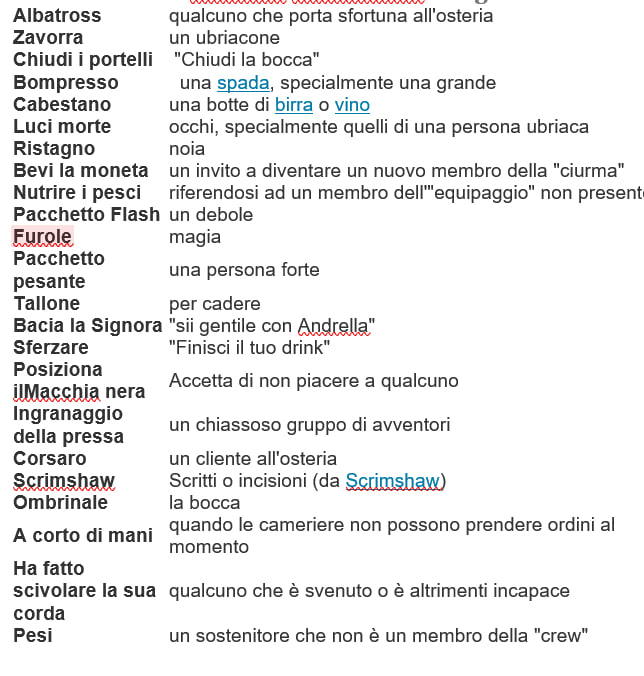
\includegraphics[width= 15cm,height = 12 cm ]{../Utilita/linguaggiodelLeviatanoSpiaggiato.jpg}
\end{figure}

Servizi\newline
Dopo la sua apertura, il Leviatano Spiaggiato divenne il luogo più popolare di Neverwinter per bere e giocare d'azzardo. La taverna ospitava spesso gruppi di intrattenitori che si esibivano nella "stiva" e sul "ponte". Quando questi intrattenitori si esibivano sul "ponte", chi si trovava nella taverna poteva sentire la musica da qualsiasi punto della nave.

Oltre a far divertire i suoi avventori, il Leviatano spiaggiato era anche sede di molti affari loschi, sia legali che illegali. In qualsiasi momento, gli abitanti di Neverwinter si riunivano qui per concludere accordi commerciali, intermediare beni rubati, scambiare informazioni di ogni tipo o per complottare. Gli affari che si svolgevano nella taverna raramente passavano inosservati agli agenti di Dagult Neverember, che frequentavano il bar a tutte le ore.

Un tipo di birra ambrata, giustamente chiamata Leviathan ale, era la birra della taverna. Una delle bevande speciali servite al Leviatano Spiaggiato era il Dwarven Celebration Brew, noto anche come "Liquido del Coraggio". Tra i cibi offerti, gli ospiti potevano assaggiare torte speziate delle Montagne della Spada, uno strano ed esotico stufato di ragno di Neverwinter, teniamo le pancette da viaggio e ordiniamo il banchetto del viaggiatore da portare via\newline\newpage
\textbf{\title{PNG}}\newline\newline
 \hypertarget{harrag}{\textbf{Harrag}} (Guerriero Liv 9)\newline
In età avanzata, Harrag era un uomo magro ma con una pancia molto pronunciata, che aveva perso una gamba in un combattimento contro i sahuagin durante i suoi anni da pirata.
\textbf{Personalità}:
Durante gli anni della giovinezza, Harrag era descritto come un uomo senza scrupoli. In età avanzata, nonostante l'aspetto burbero, Harrag era un uomo molto compassionevole e trattava i clienti abituali della sua taverna come compagni leali e fidati. Era anche descritto come un tagliagole quando faceva affari. Si vantava di essere uno spirito libero e si faceva sentire quando qualcuno insinuava che fosse il lacchè di un'altra persona. Allo stesso modo, era noto per allontanare chi si avvicinava troppo a lui.\newline\newline

\hypertarget{len}{\textbf{Len-jes}} (Elementale dell'acqua, Cugina di Umi)
\textbf{Descrizione}
Len-jes era nota per le sue cicatrici.
\textbf{Personalità}
Len-jes sembrava essere calma e raccolta, ma in realtà la furia del Caos Elementale ardeva in lei.
\textbf{Attività}
Len-jes era l'ammiraglio, il capo dell'erario e il contabile di Neverwinter. In qualità di maestro del commercio di Neverwinter, era fondamentale per far fluire il commercio nella città.

\textbf{Abilità}
Len-jes era una "idromante", quindi le sue capacità erano più forti di quelle dei normali genasi watersoul. Aveva la reputazione di essere una potente combattente.

\textbf{Storia}
Anni prima del 1479 DR, Len-jes era una corsara nel Mare delle Stelle Cadute. Tuttavia, i suoi nemici la costrinsero a fuggire e a nascondersi a Waterdeep. Nella Città degli Splendori, Len-jes fu contattata da Dagult Neverember, che la assunse come capitana di porto di Neverwinter. Nel 1479 DR, divenne una residente semipermanente del Leviatano spiaggiato. Durante i disordini civili causati dal presunto "erede perduto di Alagondar", Len-jes si schierò con i lealisti di Neverember.

\textbf{Voci di corridoio}
La gente non era sicura della vera lealtà di Len-jes. Molti credevano che lavorasse sotto copertura per i Thayan, gli Ashmadai o per i pirati di Laerakond, mentre altri credevano che fosse un'agente di Harper. Per altri, invece, era solo una lacchè assetata di potere di Neverember.\newline\newline

\hypertarget{umi}{\textbf{Umi}} (Elementale di Acqua, Cugina di Len)
Descrizione 
Simile a Len-jes
Attività
Umi era conosciuta come la "timoniera" del Leviatano Spiaggiato perché era come il garante non retribuito della taverna. Quando le cose andavano fuori controllo, Umi aiutava a calmare le risse e ad allontanare i clienti problematici. Ogni volta che sedava una rissa veniva ricompensata con drink gratuiti per la serata. Si prese cura anche di Harrag, il proprietario del Leviatano Spiaggiato, cercando di proteggerlo dalle trame di Dagult Neverember quando possibile. Umi era coinvolta anche in attività meno gustose. Ha servito come persona di contatto per molti tipi di affari illegali a Neverwinter.\newline\newline

\hypertarget{bob}{\textbf{Bobrik}}
Nano corpulento
Attività
Bobrik era conosciuto come il "nostromo" del Leviatano Spiaggiato, perché era un punto fisso della taverna e passava tutto il tempo a bere. Bobrik era rispettato e temuto dagli altri avventori per il suo caratteraccio, e solo il proprietario del Leviatano Spiaggiato, Harrag, osava chiamarlo "il nostromo" a voce alta.
Curiosità
Bobrik aveva una scimmia da compagnia che aveva chiamato "Scimmia".

\hypertarget{mark}{Markul}
umano, media statura, vestiti modesti e capelli marroni sui 60 anni
Attività
Markul era conosciuto come la "vedetta" del Leviatano spiaggiato perché trascorreva il suo tempo vigilando su tutto ciò che accadeva nella taverna. Poiché era a conoscenza di molti avvenimenti del Leviatano spiaggiato, alcuni avventori preferirono corromperlo per comprare il suo silenzio. Nessuno osava chiamarlo in faccia "la vedetta", e di solito solo i membri dello staff usavano quel soprannome per riferirsi a lui, sempre in tono basso.

La gente non sapeva che Markul era in realtà una delle persone più ricche di Neverwinter e il mecenate di molti degli affari più squallidi che si svolgevano nella taverna.\newline\newline

\hyperlink{et}{\textbf{Ettain}}
Ettain era conosciuto come il "saldatore" del Leviatano Spiaggiato perché era responsabile della manutenzione delle infrastrutture della taverna. Era anche uno dei falegnami più abili che vivevano a Neverwinter intorno al 1479 CV.
In quanto tale, Ettain conosceva ogni centimetro del Leviatano Spiaggiato ed era a conoscenza della stanza segreta in cui Harrag, il proprietario del Leviatano Spiaggiato, aveva conservato la sua fortuna personale. Ettain era un vero amico di Harrag e non tradì mai la sua fiducia. Inoltre, era una delle poche persone che cercavano sempre di proteggere Harrag dalle trame di Dagult Neverember.
\newline

\hypertarget{kor}{\textbf{Korin}}
Draconide di media statura, mingherlino, suona il violino, pantaloni attillati, bandana rossa e piercing al naso
\textbf{Le attività}
Korin era conosciuto come il "cantore" del Leviatano Spiaggiato perché si esibiva sempre nella taverna. Korin era un tipo amichevole, felice di raccontare storie e di cantare canzoni da bere e melodie marine. In alcune occasioni, ha cantato una cupa nenia su un uomo che ha perso la sua famiglia a causa di cultisti del diavolo, dimostrando un vero talento.
\textbf{Storia}
In un momento precedente al 1479 DR, la famiglia di Korin fu uccisa da cultisti Ashmadai che operavano a Neverwinter. Korin andò a vivere a Neverwinter nella speranza di rintracciare i cultisti e vendicarsi.

\subsubsection{Taverna Driftwood}

\textbf{Servizi forniti}
Bevande, pasti, camere
La Taverna Driftwood era una raffinata locanda e taverna, che fungeva anche da museo, situata nel distretto di Blacklake di Neverwinter tra la fine del 14° e la fine del 15° secolo DR. Nella seconda metà del 1400 DR, era gestita da Madame Rosene.
Descrizione
Si trovava all'interno di una torre parzialmente crollata.


\textbf{Interno}
La taverna Driftwood era decorata con curiosità, oggetti di recupero e cimeli provenienti da tutta Neverwinter prima della sua devastazione. Una vecchia statua di un'amata fontana si trovava agli angoli, le fioriere di un vinaio di Neverwintan erano montate sulle pareti e riempite di fiori, porte ornate prese dalle macerie fungevano da tavoli raffinati, la porta della latrina sfoggiava il pomello e il battente della casa di un nobile e lastre intatte di vetro colorato erano appese al soffitto e caricate con centinaia di candele da usare come lampadari. Il tutto appariva di buon gusto piuttosto che pacchiano. Gli avventori della Taverna Driftwood ritenevano che questo fosse il modo giusto per onorare il passato della Città delle Abili Mani. Rosene avrebbe rifiutato qualsiasi oggetto offerto che non riteneva degno.

\textbf{Atmosfera}
Il locale si rivolgeva a una clientela più ricca rispetto ad altri locali simili di Neverwinter e i suoi clienti erano in gran parte avventori di lunga data, cittadini e amici. Sia i nobili di Neverwintan che quelli di Waterdhavian, compresi i Margaster, potevano essere visti nella sua sala comune. I mercenari di Mintarn lo evitavano a favore di locali più economici. Inoltre, i visitatori di Neverwinter venivano qui per osservare le reliquie di Neverwintan e conoscere la vecchia città.

Si trattava di un luogo di pacifica contemplazione, non di baldoria, ma anche queste cose non erano sconosciute.

\textbf{Servizi}
Bevande, pasti e camere erano piuttosto costosi nella taverna Driftwood intorno al 1479 DR. Si potevano anche ascoltare storie sulla vecchia Neverwinter da Madame Rosen, almeno dopo aver pagato le bevande e i pasti.\newline
\textbf{Madame Rosene} Maga di settimo livello, donna affascinante ben vestita sui 50
Personalità
Madame Rosene era lenta a fidarsi degli estranei, preferendo avere a che fare con gli abitanti di Neverwinter che vivevano lì da prima dell'eruzione del Monte Hotenow.

Attività
Oltre a essere la proprietaria della Taverna Driftwood, era anche la leader della fazione conservatrice del movimento insurrezionale dei \hyperlink{alagondar}{Figli di Alagondar}, i Graycloack.

\subsubsection{Castello di NEver}
Proprietario: \hyperlink{https://forgottenrealms.fandom.com/wiki/Dagult_Neverember}{Dagult Neverember}

\textbf{Struttura}
Navigare verso Neverwinter
Il Castello di Never sovrasta la città vista dal Mare delle Spade.

Le alte e scintillanti torri del Castello Never erano la prima cosa che i visitatori che arrivavano via mare vedevano di Neverwinter. Si trattava di un edificio in pietra di imponente statura, che testimoniava le conquiste architettoniche della città. Il castello era circondato da una strada circolare e i tre ponti simbolo della città - il Delfino, il Wyvern Alato e il Drago Dormiente - si irradiavano da esso per collegarsi al distretto sud-occidentale della città.

Il Castello fu pesantemente danneggiato dall'eruzione del Monte Hotenow durante la Rovina. Metà delle sue torri si sgretolò, il muro occidentale crollò e i cortili furono disseminati di statue rovesciate e pezzi di pietra caduti. Essendo costruito su solide fondamenta, tuttavia, il resto del castello è rimasto per lo più intatto. Nel 1489 DR, il Castello Never era ancora in rovina, ma negli anni successivi sarebbe stato sgomberato e in gran parte ricostruito.

\textbf{L'interno}
L'interno del Castello Never era costituito da lunghi corridoi, eleganti cabine e sale di ritrovo. Conteneva anche spazi più utilitari, come le celle delle prigioni e un'armeria dove venivano conservate e forgiate le armi.

Durante la Rovina, gli incendi hanno spazzato via l'interno del castello, lasciandolo pieno di cenere e polvere che vorticava intorno a qualsiasi esploratore o mostro che si aggirava per i corridoi silenziosi. Mentre molte stanze erano crollate, altre erano rimaste intatte, a volte in modo inquietante, comprese alcune delle aree più fortificate del castello, in particolare l'armeria, la sala grande e le segrete. L'intero luogo puzzava di cenere e i lamenti e i singhiozzi degli spiriti morti durante l'eruzione riecheggiavano nelle sale. Le torri e i piani superiori erano ricoperti di ragnatele alla fine del XV secolo.

\textbf{Atrio}
Durante il periodo di massimo splendore della famiglia Alagondar, il castello conteneva un giardino all'aperto e una voliera. Conteneva una bella collezione di fiori e altre piante, oltre a splendidi uccelli in gabbie ornate. Dopo la Rovina, sia le piante che gli uccelli furono lasciati marcire e l'atrio fu invaso da aggressivi miconidi nati dalle spore di qualcosa della collezione di piante. Alla fine del XV secolo DR era riuscita a sigillare completamente il tetto, un tempo aperto, intrappolando l'odore di marciume e le fioriture di funghi all'interno.

\textbf{Sala Grande}
La Sala Grande del castello era arredata in marmo con un tappeto rosso e ospitava il trono del sovrano della città. La sala conteneva antiche difese magiche che davano l'allarme e sigillavano il cancello se il castello veniva attaccato.

\textbf{Sala degli specchi}
Questo lungo corridoio, con un'enorme finestra su un'estremità, era ornato da specchi a figura intera e veniva utilizzato dalla famiglia reale per esercitarsi nella postura e nell'aspetto. Tuttavia, quando il Monte Hotenow eruttò, questo si rivelò uno dei luoghi più terribili del castello: prima gli specchi si frantumarono, riducendo in pezzi tutti gli occupanti, prima che i gas vulcanici brucianti attraversassero la finestra e incenerissero i corpi. La ferita spirituale lasciata dalle vittime ha fatto sì che la cenere e il vetro della stanza si animassero e rievocassero lentamente l'evento ogni volta che un essere vivente entrava nella stanza. A quel tempo era nota anche come Sala degli Specchi di Cenere.


\textbf{Il caveau}
I tesori del Castello Never e dei suoi occupanti erano conservati in un caveau sicuro, noto per essere uno dei luoghi più protetti della Costa della Spada. Le saracinesche alle finestre e un allarme che mobilitava rapidamente le guardie dovevano garantire che nessun ladro che si fosse avvicinato al caveau sarebbe riuscito a fuggire. Alla fine del 1490, la porta del caveau era protetta dal sigillo arcano di Mordenkainen.

\textbf{Neverneath}
Conosciuto anche come il "Labirinto senza fine", Neverneath era il complesso di catacombe del Castello Never, contenente una prigione fortificata e vaste cripte, come la tomba di Lord Halueth Never. Queste catacombe erano protette magicamente per mantenere l'integrità strutturale dell'edificio sovrastante, ma la Peste Incantatrice ha alterato nel tempo la protezione magica, aumentandone il potere e conferendole una sensibilità malevola e la capacità di rimodellare i corridoi di Neverneath a piacimento per confondere e intrappolare gli intrusi. I corridoi potevano riavvolgersi su se stessi, formando anelli infiniti pieni di trappole mortali e gargoyle che attaccavano qualsiasi cosa si muovesse. Si dice che nelle profondità delle viscere del Neverneath vi siano collegamenti con lo Shadowfell e con l'Underdark.


\textbf{Tomba di Halueth Never}
Nelle profondità del castello si trovava l'ultima dimora di Lord Halueth Never. Il suo corpo giaceva su una grande lastra di pietra ed era protetto da un anello di dodici spade incantate e scintillanti che si sarebbero animate e avrebbero attaccato qualsiasi intruso se non avesse seguito le istruzioni criptiche scritte sulle lastre. Era inoltre protetto dalle statue incantate dei suoi servitori più fidati, tra cui quelle dei nove Neverwinter originali.

\textbf{Cripta dei Nove}
I Nove di Neverwinter, nove guardie del corpo d'élite di Nasher Alagonadar e difensori della Casa Alagondar, sono stati sepolti in una cripta sigillata magicamente nelle profondità del Neverneath. Quest'area consisteva in una camera circolare di 61 metri di diametro, riempita di torce sempre accese, che circondava una volta interna sigillata con il sigillo di Neverwinter e protetta da una potente magia. All'interno, la Volta Interna era scolpita con immagini idilliache dell'Estate, illuminate da una luce fioca che irradiava da nove bare di marmo disposte a raggiera intorno a un trono d'oro.

\textbf{Le buche}
Quando il Castello Never fu sgomberato e tornò in uso alla fine del XV secolo, una sezione sotto le rovine fu adibita a prigione per i criminali condannati a morte per crimini gravi, tra cui l'omicidio e il tradimento (compresa l'evasione fiscale). Questo sotterraneo, noto come "i buchi", era pesantemente sorvegliato e ospitava esecuzioni di massa una volta ogni giorno, in cui i condannati venivano impiccati pubblicamente. Ai prigionieri era concesso un ultimo pasto consegnato da amici e familiari il giorno prima della loro morte, ma per il resto chiunque fosse stato sorpreso a entrare nelle buche veniva condannato alla reclusione anche in esse. La prigione era accessibile solo attraverso un'unica entrata, pesantemente sorvegliata, situata al livello principale del castello, anche se si vociferava di un tunnel segreto infestato da mostri che collegava le buche alla riva del Blacklake.


\textbf{Le attività}
Prima della Rovina, il castello era la sede del signore di Neverwinter. Nel 14° secolo d.C., regnanti come Nasher Alagondar ricevevano i visitatori. Alla fine del 15° secolo d.C., Dagult Neverember aveva restaurato il castello a sufficienza per potervi tenere nuovamente corte.

\subsubsection{PiùSoldiPiùPrestiti}
Descrizione
PiùSoldiPìùPrestiti era un negozio specializzato nel commercio di valuta. Per una piccola somma, le persone potevano cambiare il denaro da e verso una valuta diversa. Il negozio era pesantemente protetto da orrori elmati.


\subsubsection{Casa delle Mille Facce}
Proprietaria: \hyperlink{ther}{Theryis} \newline
la Casa dei Mille Volti era una taverna situata nel Distretto di Blacklake di Neverwinter. Era il quartier generale degli Arpisti di Neverwinter negli ultimi anni del 15° secolo DR.
Descrizione
L'edificio prendeva il nome dai numerosi specchi e manichini posizionati nella sala comune. C'erano tre ingressi alla Casa, due sul lato nord e uno sul lato sud, e molti specchi e manichini erano posizionati intorno ad essi, invitando gli avventori ad entrare. Tutti i manichini erano vestiti secondo la moda popolare a Neverwinter negli ultimi anni del XIV secolo.

Inoltre
Oltre a essere una taverna, la Casa dei Mille Volti era anche una locanda. Una notte nella Casa costava 1 mo per ospite.

\hypertarget{ther}{\textbf{Therysis}}
Personalità
Theryis era una persona serena e comprensiva, in contrasto con la personalità del fratello.

Relazioni
Theryis era la sorellastra di Toram.

Capacità
Theryis era un'arciera arcana.[

Attività
Oltre a essere un'Arpista, Theryis era anche proprietaria e amministratrice della Casa dei Mille Volti.

\subsubsection{Accademia della Stella Splendente}
\textbf{Servizi}
L'Accedemia delle Stella Splendente insegnava ai suoi studenti a creare e apprezzare l'arte, oltre che a conoscere le erbe, le conoscenze e le abilità agricole e a conoscere gli animali selvatici in base all'odore, al suono e alle tracce. La scuola vendeva anche dipinti, erbe, ricette, disegni di riferimento per gli animali e pozioni curative.

Tuttavia, la scuola si rivolgeva anche a persone che volevano imparare a preparare pozioni più pericolose, come quelle che inducevano il sonno, l'aumento delle sensazioni o la lussuria. Si diceva anche che la scuola vendesse anche veleni.

\subsubsection{Villa Vellgard}
\hyperlink{mor}{\textbf{Mordal Vell}} (Ladro, Livello 6)
Descrizione
Il maniero era fiancheggiato da cancelli di metallo e da un muro interno in grado di fermare un piccolo esercito.

Storia
Mordai Vell ereditò il maniero dopo l'eruzione del Monte Hotenow, nel 1451 DR, quando tutti i suoi parenti umani morirono nel cataclisma. In seguito ha riadattato il maniero per utilizzarlo come quartier generale della sua cellula \hyperlink{ash}{Ashmadai}.\newline

\hypertarget{mor}{Mordal Vell}
Personalità
Era affascinante e manipolatore e aveva un ruolo in molti avvenimenti di Neverwinter. È stato anche descritto come "l'arroganza incarnata" a causa del suo comportamento.

Attività
Vell era il capo di una delle cellule Ashmadai che operavano a Neverwinter, ma le sue interpretazioni dei principi e degli editti di Asmodeus erano piuttosto liberali. Vell vedeva il suo servizio al dio dei Nove Inferi come un mezzo per raggiungere un fine, piuttosto che servire un padrone.

Possedimenti
Vell era il proprietario di Vellgard Manor, una villa nobiliare nel distretto di Blacklake a Neverwinter.

\subsubsection{Il Liuto Muto}
Rebeth Laereeryn mezzelfo
con un incantesimo può impedire che tutti i suoni provenienti dall'interno del suo negozio si diffondano all'esterno, se lo desidera.
Descrizione
Il Liuto Muto era popolare in tutti i Regni per i suoi liuti ben fatti. Il negozio era costruito attorno a una vecchia quercia. Il nome del Liuto Muto deriva da un incantesimo che la sua proprietaria, Rebeth Laereeryn, poteva lanciare per far tacere tutti i suoni all'interno delle sue mura.

Prezzi
I liuti comuni del Mute Lute costano 900 mo, mentre quelli fatti su misura possono costare fino a 3000 mo.

\subsubsection{Le meraviglie meccaniche di Dannar}
Descrizione
Le Meraviglie Meccaniche di Dannar era un negozio specializzato in costosissimi congegni a orologeria gnomici, lantani e nani. Ne erano un esempio le scatole di pietra focaia a carica automatica e a pulsante e i portagioie in electrum intarsiati di perle e dotati di ornamenti animati, come piccoli draghi a orologeria che rincorrevano le loro code attorno a uno specchio di vanità a scomparsa. Questi oggetti tendevano a stupire i visitatori.


\subsubsection{Opere in porcellana Fineware di Jaesor}

Proprietario: Jaesor Ryndyl

Descrizione
Jaesor's era un negozio specializzato in lavori di porcellana. Questo negozio era popolare tra le famiglie famose di Neverwinter negli ultimi anni del 14° secolo.

Prezzi
Un piatto dipinto su misura costava 20 mo, mentre un set di 20 pezzi costava 45 mo.

\subsection{Enclave dei Protettori}
\subsubsection{Casa del Commercio di Tarmalune}Descrizione
La Casa del Commercio aveva un grande magazzino situato nel Distretto dei Docks per immagazzinare le proprie merci. Disponeva anche di un punto d'asta all'aperto situato nell'Enclave del Protettore.

I mercanti di Tarralune utilizzavano un tipo di moneta unico, i Barre del Commercio di Tarmalune, fatti d'argento e con impressi i marchi commerciali di Tarralune. I lingotti potevano essere scambiati con equipaggiamento, cavalcature, contratti di avventura e altri oggetti di valore.
\subsubsection{Sala della Giustizia}
Personale
\title{\textbf{Soman Galt}} 1467 DR-oggi\newline
Personalità
A causa di un forte condizionamento mentale, Galt era una persona introversa, solitamente persa nei suoi pensieri e che borbottava tra sé e sé. Tuttavia, era in grado di mostrare una sorprendente capacità di concentrazione quando doveva concentrarsi su qualcosa, e prendeva sempre sul serio il suo lavoro.

Era consapevole che Neverember lo considerava solo un lacchè, ma non gli importava, perché era un fedele servitore dei suoi veri padroni. Quando gli veniva ordinato dagli Abolitici, o quando la sua vita era in pericolo, Galt poteva diventare molto aggressivo e si preoccupava solo della distruzione.

Attività
In qualità di sindaco di Neverwinter, Galt era responsabile del governo quotidiano di Neverwinter.

Era anche un fantoccio della Sovranità Abolitica e il suo ruolo era quello di informare i suoi padroni di qualsiasi evento importante e di influenzare il governo di Neverwinter in modi che fossero vantaggiosi per gli Abolitici.

La storia
In gioventù, Galt era un abile esploratore e funzionario del governo. Grazie alla sua esperienza, fu scelto da Dagult Neverember come sindaco di Neverwinter quando questi diede vita al movimento Nuova Neverwinter nel 1469 DR.

A un certo punto, prima del 1479 d.C., Galt fu avvicinato da Rohini, che lo sedusse e riuscì a mandarlo dai suoi padroni, la Sovranità Abolitica, che controllò e modificò Galt per servirlo come loro burattino a Neverwinter.


Mercenari di Mintarn, Sacerdoti di \hyperlink{https://forgottenrealms.fandom.com/wiki/Torm}{Torm} e \hyperlink{https://forgottenrealms.fandom.com/wiki/Tyr}{Tyr}
\newline


\title{La posizione}\newline
La Sala della Giustizia si trovava su una scogliera che dominava il Mare delle Spade, sulla riva meridionale del fiume Neverwinter, vicino alla sua foce. Si trovava proprio di fronte al Ponte del Drago Dormiente dal Castello Never.

Prima della Rovina del 1451 DR, la Sala della Giustizia si trovava nel Nucleo della città, mentre dopo gli sforzi di ricostruzione degli ultimi anni del decennio 1470 DR, si trovava nell'Enclave del Protettore.\newline

\title{La struttura}
La chiesa, scintillante e simile a un castello, era costruita in pietra, ferro e legno ed era imponente ma bella da vedere. Era un edificio grandioso che poteva ospitare comodamente i giganti e nella sua grande sala c'era spazio sufficiente per far riposare i draghi.\newline
\title{Interni}
La chiesa si distingueva per gli alti soffitti, ma era decorata in modo sobrio, con diverse stanze per la routine quotidiana e il culto. Il sommo sacerdote aveva un proprio appartamento nel tempio.
\subsubsection{Tomba di Traditori }
Notevoleoccupanti
Fenthick Moss (Era l'amante di \hyperlink{https://forgottenrealms.fandom.com/wiki/Aribeth_de_Tylmarande}{Aribeth de Tylmarande.}) Chierico 6 livello
La Tomba dei Traditori era una cripta a Neverwinter, sulla Costa della Spada.
UbicazioneLa tomba si trovava a Neverwinter, vicino alla Chiesa di Tyr.

\textbf{Struttura}
Una tomba di pietra, composta da tombe vicino all'ingresso.

\textbf{Interno}
La tomba era composta da diverse sale e stanze, sorvegliate da non morti e con molte trappole.
\subsubsection{Torre della Pesta}
Proprietario : Rhazzad (Mago, Elfo della Luna) \newline
Occupanti: Piaga \newline
Servizi forniti
Trattamento per gli appestati
La Torre della Pace, in seguito nota come Torre della Peste, era una grande torre che si trovava nella città di Neverwinter durante il XV secolo DR.
\textbf{"Non siamo più come prima, ma siamo ancora insieme"
- Iscrizione sulle statue della Fanciulla, della Madre e della Cora.}
Ubicazione\newline
La torre si trovava nell'Enclave dei Protettori, oltre il ponte a sud-est del Castello Never.

Struttura\newline
La torre aveva una forma circolare, con un corridoio esterno semicircolare che circondava una camera centrale a colonne. Le doppie porte dell'ingresso principale della torre si trovavano in cima a una piccola scala quadrata, che apriva al secondo livello dell'interno.

Sotto la torre stessa si trovava una serie di passaggi cavernosi, utilizzati principalmente come magazzini.\newline
L'interno\newline
Statua della torre
La statua rotta della torre è rimasta "intatta" con mezzi sconosciuti

Entrando nella torre al secondo livello si accedeva al corridoio esterno semicircolare, all'interno del quale si trovava una camera circolare che si estendeva per tutta la torre fino all'ultimo piano. All'interno di questa sala centrale si trovava una grande scala doppia a spirale che si snodava fino ai numerosi piani della torre. La doppia scala circondava una massiccia statua di quella che sembrava essere una donna elfica con ali piumate e il corpo di un serpente.

Un tema artistico comune a tutta la torre era una serie di statue di pietra chiamate la Fanciulla, la Madre e la Cora. Si trattava di figure femminili di età variabile, che portavano rispettivamente un fiore, una cornucopia e un bastone. Ogni statua, in ogni luogo, poteva essere regolata sulla sua predella per essere rivolta verso le quattro direzioni cardinali.

Se si allineano le tre statue nella direzione corretta, si apre un passaggio nella torre.

L'atmosfera\newline
La torre aveva un'architettura spaziosa e austera, con grandi corridoi fiancheggiati da colonne di pietra e cancelli interni di ottima fattura. Le pareti erano decorate con una serie di grandi arazzi e all'ultimo piano c'erano persino finestre con vetri colorati. L'interno della torre possedeva una certa sensazione di raffinatezza e austerità.\newline
Attività\newline
Sebbene non si conosca l'abitante originario della torre, questa era stata adibita a torre dei maghi dal malvagio incantatore Rhazzad. Trasformandola in quella che divenne nota come "Torre della Peste", il mago elfico condusse esperimenti sugli abitanti di Neverwinter modificati dalla peste.

\subsubsection{Armi artigianali e armi magiche di Allis Lhyssich per nobili cause}
Proprietario/i
Allis Lhyssich (umano, devoto a Tyr): Lhyssich era famoso per essere in grado di lavorare con i rari minerali di meteorite e di ricavarne armi incantate. Gli è stata attribuita la creazione della spada del taglio della pietra, una spada magica eccezionale per combattere le creature malvagie e quelle fatte di pietra.\newline
Armi artigianali e armi magiche di Allis Lhyssich per nobili cause era un negozio specializzato in armi che vendeva anche equipaggiamento standard.
Ubicazione
Il negozio si trovava vicino al cancello sud di Neverwinter.
\textbf{Servizi}
Il maestro fabbro, Allis Lhyssich, era uno dei pochi in grado di creare armi magiche con il minerale di meteorite. La procedura di lavorazione richiedeva tre giorni per realizzare queste armi di meteorite altamente incantate.
\subsubsection{Cripte della Gilda dell'Orologio ad Acqua}
Descrizione
Il mausoleo era un complesso di ingranaggi, cascate e trappole, alimentato da elementali dell'acqua legati a mantenere in funzione le macchine per secoli. L'acqua del mare scorreva attraverso vene traslucide nelle pareti, riversandosi verso Luskan e Gauntlgrym.
\subsubsection{Cimitero - Neverdeath}
Descrizione
Costituita da due ampie aree della città, approssimativamente quadrate, e circondata da un muro di pietra e legno, Neverdeath era il luogo di sepoltura di Neverwinter. Il nome deriva da una benedizione comune impartita ai morti. Finché la città rimaneva in estate, si credeva che i morti non si sarebbero trasformati in non morti.
Le guide del destino dell'Ordine Eterno di Kelemvor erano responsabili della protezione di quest'area.
\subsubsection{Armi e armature del Cavaliere Splendente}
Descrizione
Armi e armature del Cavaliere Splendente era una delle migliori armerie di Neverwinter, perché il suo proprietario era un mago che conosceva gli incantesimi che lo aiutavano a modellare il metallo, e che lavorava anche con i nani per creare buone armi e armature.
\subsubsection{il Muro}
Descrizione
La Barriera fu costruita con pietre, legno e altri materiali presi dalle macerie di Neverwinter. Si estendeva dal cimitero di Neverdeath fino alla Casa della Conoscenza e al fiume Neverwinter. Gran parte della Barriera era costituita da ex manieri, torri e persino da una delle antiche caserme della Guardia. Era abbastanza grande da sovrastare gli altri edifici della città.

La Barriera era presidiata dalla Guardia di Neverwinter. Gli avamposti attraverso la Barriera erano sempre sorvegliati da almeno dieci guardie e gruppi di soldati e mercenari pattugliavano costantemente la Barriera da un capo all'altro, giorno e notte.

\subsubsection{Casa della Conoscenza}

Reggente: \textbf{Spivey Liethennsonc} 1496 DR
descrizione\newline
Era il sacerdote capo che presiedeva sia il tempio che la biblioteca della Casa della Conoscenza, e veniva descritto come un leader dal pugno di ferro. Era fragile, sia nel corpo che nel temperamento, e il suo respiro era pesante e affannoso.

Pur essendo più un amministratore che un incantatore, Liethennson era noto per occuparsi della rimozione di maledizioni come la licantropia come parte dei suoi compiti nel tempio.\newline

Personalità\newline
Liethennson era molto esigente nei confronti dei suoi sottoposti ed era noto per le sue lamentele e i suoi continui rimproveri per eventuali mancanze o carenze. Si arrabbiava rapidamente e raramente era gentile.\newline

Storia
Liethennson arrivò a Neverwinter probabilmente alla fine del 1480 d.C., quando la Chiesa di Oghma si impegnò a inviare membri del clero per restaurare la Casa della Conoscenza,[2] che era stata gravemente danneggiata durante la Rovina del 1451 d.C.[3] A metà del 1490 d.C., era responsabile dell'intero tempio e forse il suo ruolo più importante in questo periodo fu la gestione della ricostruzione. Nel 1496 d.C. le pareti esterne del tempio erano state completamente ricostruite, ma i lavori continuavano all'interno e all'arredamento. Durante questo periodo, il suo atteggiamento irritante fece sì che Kollette Kwarter e la sua squadra, i costruttori che supervisionavano la ricostruzione, abbandonassero il progetto.\newline

Occupanti
Chiesa di \hyperlink{https://forgottenrealms.fandom.com/wiki/Oghma}{Oghma}, rifugiati spellscarred (fino alla fine del Secondo Assolvimento), Ashmadai
Divinità patrona
Oghma
La Casa della Conoscenza, nota anche come Sala della Conoscenza, era una biblioteca e un tempio di Oghma, il Legatore di ciò che è noto, nella città di Neverwinter della Costa della Spada Nord tra la metà e la fine del 14° e la fine del 15° secolo DR.
Ubicazione
Si trovava vicino al lato meridionale del Ponte dei Delfini, all'interno del distretto dell'Enclave del Protettore, all'estremità nord-orientale della Barriera, alla fine del 1400 DR. Una strada tortuosa che corre a sud-est della Casa della Conoscenza ospitava molti librai, rilegatori e scribi nel 1300 DR; uno di questi era Mappe e Leggende di Maskado.

Struttura\newline
La Casa della Conoscenza era considerata uno degli edifici più imponenti di Neverwinter, una città la cui fama si era diffusa in tutta la Costa della Spada. Si trattava di un edificio imponentemente alto, con molte finestre e un tetto ad arco.

Dopo l'eruzione del Monte Hotenow nel 1451 d.C., la Casa della Conoscenza fu gravemente danneggiata e, alla fine del 1470 d.C., si trovava ancora in rovina, con le finestre di vetro rotte e un aroma di tomi polverosi ed erbe medicinali, a causa della sua ristrutturazione. I lavori di riparazione iniziarono intorno al 1489 d.C. e si protrassero fino alla metà del 1490 d.C., quando i muri e i pavimenti esterni furono completamente restaurati. I lavori proseguirono per le pareti interne e l'arredamento.

L'interno\newline
Il santuario principale di Oghma si trovava al piano terra ed era aperto al pubblico. Al piano superiore si trovavano le aree di soggiorno del personale del tempio, gli uffici e i laboratori, mentre nel seminterrato si trovavano i magazzini e altri santuari per il culto privato.

La Casa della Conoscenza era anche una grande biblioteca, che conteneva di tutto, da mappe e storie a poesie e letteratura. I libri comuni e le pergamene, compresi i documenti del governo pubblico, erano ospitati al primo piano, mentre nel sottosuolo si trovava una biblioteca più sicura, nota come la Volta dei Tomi, dove erano conservati alcuni dei libri più rari e preziosi non presenti a Candlekeep. La Volta era ben sorvegliata e dotata di una complessa serratura a tre livelli, che la rendeva uno dei luoghi più sicuri di Neverwinter.
Attività\newline
Nel 1300 DR, il tempio offriva istruzione gratuita, con sessioni di insegnamento che raddoppiavano i servizi al Binder. Era una grande biblioteca che comprendeva storie, mappe, poesie e libretti scritti nel corso dei secoli.

In seguito all'eruzione del Monte Hotenow, tuttavia, alla fine del 1400 DR, il tempio servì come campo profughi e ospedale di fortuna, fornendo cure ai guardiani di Neverwinter feriti e alle persone colpite dal Baratro, nonché vitto e alloggio ai viaggiatori che davano una mano.

Nel 1490 DR era tornato a essere un luogo di apprendimento e un deposito di informazioni, oltre che un luogo di incontro.



\subsection{Extra}
\subsubsection{Maschera in pietra di luna}
Proprietaria : Liset Cheldar
Relazioni
Liset ha affermato di essere un discendente di Ophala Cheldarstorn.[1]

Descrizione\newline
Nel 1479 DR, Liset era una donna di mezza età.[2]

Personalità\newline
Liset cercava di prendersi cura dei suoi ospiti, era amichevole e le piaceva flirtare con gli uomini che la incuriosivano.

Attività\newline
Liset è stata una delle poche sopravvissute all'eruzione del Monte Hotenow. Fuggì dalla città dopo la distruzione di Neverwinter.

Qualche tempo prima del 1479 DR, Liset si avvicinò a Lord Dagult Neverember e lo convinse a permetterle di reclamare la sua eredità, la locanda Moonstone Mask nell'Enclave del Protettore. Lo convinse anche a sponsorizzare la riapertura della locanda.

A partire dal 1479 DR, era piuttosto popolare tra i mercenari di Mintarn assunti da Lord Neverember.

Voci di corridoio\newline
Alcuni ritenevano che Liset avesse sedotto Neverember per convincerlo ad aiutarla a reclamare e riaprire la Maschera.

Alcuni ritenevano anche che Liset lavorasse per forze sinistre, di sua spontanea volontà o costretta a farlo, e che il suo volto amichevole fosse solo una facciata. Tuttavia, le persone che credevano a queste voci non erano sicure dell'identità della forza che si celava dietro Liset: alcuni indicavano i Thayan o i Netherese, mentre altri credevano che fosse una schiava della Sovranità Abolitica.
\newline
Servizi forniti
Torte calde (dal 1366 DR)
Ottimo vino feywine e forte liquore nanico (dal 1479 DR)

Il personale\newline
Il personale era composto esclusivamente da donne che indossavano maschere luminose e bordate di pietra di luna (da cui il nome del locale) e abiti neri trasparenti. Erano conosciute come amichevoli e sagge, nonché rinomate giocatrici di molti giochi. Non rivelavano mai la loro vera identità e indossavano sempre la maschera mentre lavoravano. Questo senso di anonimato li rendeva confidenti rinomati in tutta la Costa della Spada e oltre. Tutti i membri del personale indossavano anche amuleti magici che li proteggevano dalla lettura del pensiero e dalla magia che controlla la mente e permettevano loro di inviare messaggi mentali tra i portatori di altri amuleti.

I cuochi, invece, erano tutti maschi.

Nel 1374 DR, la Maschera era di proprietà e gestita da Ophala Cheldarstorn. Nel 1479 DR, il proprietario era il presunto discendente di Ophala, Liset Cheldar.

Descrizione
La Maschera di Pietra di Luna era un edificio a cinque piani. Il primo piano era la sala da pranzo, illuminata da un enorme focolare e da lanterne appese ai lati della grande scala. I tre piani successivi avevano la particolarità di essere insonorizzati, grazie alla magia lanciata durante la costruzione della locanda. Questi piani erano dedicati all'affitto delle loro lussuose stanze ai viaggiatori e agli avventori abituali. Il quinto piano fungeva da sala delle feste. Il tetto era dotato di una piattaforma di atterraggio per i destrieri alati e le navi volanti.

Dopo la Spellplague del 1385 DR, la terra intorno alla locanda si liberò e iniziò a fluttuare nell'aria, diventando un earthmote. Per mantenere il lombrico in posizione fissa, i proprietari della Maschera commissionarono una serie di pesanti catene abbastanza grandi da tenere fermo un gigante, mentre un ponte galleggiante e instabile permetteva agli avventori di accedere da terra. Intorno al 1479 DR, Liset Cheldar commissionò un portale magico per consentire un accesso più facile e confortevole alla Maschera.

Difese
A partire dal 1366 d.C., Ophala aveva a disposizione dodici orrori da battaglia per proteggere la Maschera. Era anche un'abile e potente maga.

Intorno al 1479 d.C., la Maschera fu protetta dai suoi protettori, per lo più mercenari di Mintarn assunti da Lord Dagult Neverember.
Servizi\newline
Il Mask serviva molti tipi di piatti di carne su ordinazione, tra cui singolari pasticci caldi a base di cinghiale e vitello, pancetta e rognone, frutti di mare o fegato di pollo. Il suo piatto di spiedini Daintyfish era preparato con venti pesciolini chiamati silverflashes. I Daintyfish venivano immersi nel burro alle erbe e sfrigolati alla fiamma fino a diventare croccanti. Allo stesso modo, il Mask offriva un menu assortito di zuppa di cozze e basilico, zuppa di pesce, zuppa di tartaruga, brodo di polpo, funghi inzuppati in una salsa alle erbe e all'aglio, scalogni e finocchi immersi in un brodo di pollo al prezzemolo e alla menta. Per quanto riguarda i dolci, il Mask offriva torte di more e mele, condite con crema e mandorle a fette; uva spina grande come un palmo, crostate di mandorle e, quando era disponibile il cioccolato, fragole con una copertura di cioccolato ghiacciato.

Dal 1479 DR, una tavola di vendita permetteva di offrire lavoro a mercenari e avventurieri.
Prezzi\newline
Una camera per una notte aveva un prezzo di 16  mo, comprensivo di servizi di scuderia e di tutto il cibo e le bevande desiderati, mentre una singola cena aveva un prezzo di 10  mo. Se un cliente desiderava la compagnia di una delle dame dello staff, il conto veniva maggiorato di 45  mo.

Il vino di buona qualità costava 6 mo, il vino di fuoco 9 mo e l'elverquisst 20 mo. Un boccale di birra o sidro costava 4 mr.

A partire dal 1479 DR, Liset ha aggiunto al suo menu il pregiato feywine e il forte liquore nanico. Un bicchiere costava mo  mo, mentre una bottiglia costava 50 mo.

Una rara prelibatezza, il soufflé all'uovo di ragno, veniva servita alla locanda per soli mo  mo.
\subsubsection{Ponte del Drago dormiente}
Descrizione
Il ponte è stato scolpito con le sembianze di un drago.

Posizione
Il ponte del Drago Dormiente, insieme agli altri due ponti, si irradiava dal Castello Never, collegandolo al resto della città. Nel caso del Drago Dormiente, collegava il castello con la Sala della Giustizia.

La storia
Durante la Rovina del 1451 DR, il Ponte del Drago Dormiente fu distrutto dal cataclisma.

Nel 1479 DR, il Ponte del Drago Dormiente fu il luogo dell'ultima battaglia dell'assedio di Neverwinter.
\subsubsection{Ponte Wyvern alato}
Descrizione
Il ponte è stato scolpito con le sembianze di un wyvern. Si distingueva dal ponte del Drago Dormiente per le sue ali allungate.

Posizione
Il Ponte del Wyvern Alato, insieme agli altri due ponti, si irradiava dal Castello Never, collegandolo al resto della città. Nel caso del Wyvern alato, collegava il castello con la piazza del mercato della città.
\subsubsection{Ponte del Delfino}
Descrizione
Il ponte è stato scolpito a forma di delfino.

Posizione
Il Ponte dei Delfini, insieme agli altri due ponti, si irradiava dal Castello Never, collegandolo al resto della città. Nel caso del Delfino, collegava il castello con la Casa della Conoscenza.

La storia
Durante la Rovina del 1451 DR, il Ponte dei Delfini fu distrutto dal cataclisma.
\subsubsection{La cavità di Scalefather}
Società
Razze
Lizardfolk
La Grotta di Scalefather era una grotta tortuosa che si trovava nella palude di Vilebog a Skyhold dei Pirati.

Descrizione\newline
La caverna comprendeva una formazione naturale di grotta i cui tunnel sono stati aggiunti da influenze non naturali. Travi di legno di sostegno si trovano lungo le pareti ricoperte di muschio della grotta, così come massicce radici di alberi che si estendono nel sottosuolo dalla palude sovrastante.

I soffitti della grotta presentavano numerose aperture, che consentivano ai flussi d'acqua di scendere dalle zone umide e di accumularsi sul pavimento della caverna. Pochi di questi fori permettevano alle colonne di luce di brillare all'interno, fornendo un'illuminazione limitata in alcune aree.

Geografia\newline
Si trova nel tratto sud-occidentale di Vilebog, appena a ovest del luogo di schianto dell'astronave Magister's Hope.

Storia\newline
Scalefather's Hollow fu saccheggiata dall'Eroe del Ponte del Drago Dormiente nell'Anno dell'Eterno, 1479 DR, mentre era alle dipendenze del gruppo di mercenari della Compagnia Yargo.

Abitanti\newline
La grotta prende il nome da Scalefather, lo sciamano della tribù di lizardfolk che viveva nella palude di Vilebog.
\subsubsection{Vilebog}
Tipo
Palude
Regione
Skyhold dei Pirati, Faerûn nord-occidentale
Altezza
30 m
Società
Razze
Lizardfolk
Il Vilebog era un'ampia e pericolosa zona umida che si trovava in cima alla terramote nota come Skyhold dei Pirati, che si stagliava nei cieli della Costa della Spada settentrionale durante la RD del XV secolo.

Descrizione
La fetida palude era considerata quasi inospitale a causa della sporcizia e delle malattie che avvelenavano le sue acque. Gli sciami di insetti si rivelavano più che un fastidio per chiunque tentasse di attraversare il suo terreno ripugnante.

A un certo punto della sua storia, per facilitare l'attraversamento dei corsi d'acqua della palude furono costruiti una serie di ponti di legno traballanti, che però col tempo si sono degradati e sono caduti a pezzi.

La geografia
Vilebog
Le fetide acque del Vilebog.

La palude si trovava nel tratto occidentale del earthmote, un po' più a ovest della Fortezza del Teschio.

Caratteristiche geografiche
Non tutta la vita naturale pr
esente nel Vilebog era dannosa o tossica. Alcune rare erbe medicinali potevano essere trovate da chi le osservava con sufficiente attenzione.
\subsubsection{Ritiro del Re dei Pirati}
Altezza
30 m
Il Ritiro del Re dei Pirati, chiamato anche Covo del Re dei Pirati, era una città-fortezza costruita all'interno del globo terrestre noto come Skyhold dei Pirati. Era il dominio eterno di Bartholomew Blackdagger, il famigerato re dei pirati che terrorizzò il Mare delle Spade per oltre un decennio all'inizio del XV secolo DR prima di essere condannato alla morte eterna.

Descrizione
Tana del Re Pirata
Nelle profondità del nascondiglio del Re dei Pirati.

Il rifugio di Pugnale Nero comprendeva un piccolo e rudimentale insediamento in cima a un massiccio e labirintico forte costruito nell'isola galleggiante di Skyhold dei Pirati. Le sue semplici strutture erano costruite in pietra e malta o, più spesso, in legno e intonaco, mentre altre erano ricavate dalle carcasse di navi di legno riutilizzate.

La fortezza di pietra era di dimensioni e portata enormi e comprendeva cupe camere sotterranee interconnesse da corridoi pieni di trappole e delimitate da saracinesche di ferro. I sotterranei sotto la fortezza conducevano alle caverne naturali che si snodavano lungo il nucleo del earthmote. In tutta la rete di caverne si trovavano grotte isolate collegate da ponti di corda traballanti e grotte pittoresche nascoste dietro a cascate.

Una serie di lanterne che emettevano un fuoco blu simile a quello della Peste Incantata si trovava in tutti i passaggi intorno alla fortezza-isola volante dei pirati.

Geografia
Flora e fauna
Sia i sotterranei della fortezza che le grotte circostanti erano invase dalla rete di radici del fitto fogliame che si trova sulla superficie di Skyhold dei Pirati.

Storia
Pugnale Nero in cima al Flagello Nero
Il pugnale nero non morto che langue a bordo della Black Scourge.

A metà del XV secolo, a Bartholomew Blackdagger e alla sua ciurma fu impedito di lasciare la ritirata dopo che il re dei pirati, notoriamente avido, sfidò stupidamente il grande wyrm nero Garrundar il Vile. Dopo un assalto aereo fallito, il drago maledisse Pugnale Nero con la morte eterna, impedendogli di lasciare il suo dominio per non essere completamente disintegrato. Non volendo lasciare che sia un altro a dettare i termini della sua vita, o addirittura della sua vita ultraterrena, Pugnale Nero volle che la maledizione si diffondesse ai suoi uomini, costringendoli a rimanere avvinti a lui per sempre, mentre cercava la vendetta finale contro Garrundar.

Nell'Anno del Senza Età, 1479 DR, la vile maledizione che affliggeva i non morti del Ritiro del Re dei Pirati fu finalmente interrotta. Un gruppo di avventurieri lavorò insieme ai mercenari della Compagnia Yargo e a una banda di pirati pugnali neri ammutinati, fortunatamente risparmiati dalla maledizione che affliggeva i loro ex compagni di ciurma, per distruggere Bartholomew Blackdagger e i suoi luogotenenti una volta per tutte.

Luoghi degni di nota
Black Scourge, l'astronave personale di Blackdagger, è rimasta attraccata al Ritiro del Re dei Pirati, incapace di solcare i cieli finché è rimasto sotto la vile maledizione.
Abitanti
L'intero forte era invaso da non morti che in vita erano membri della ciurma pirata di Blackdaggers. Tra gli uomini di spicco della ciurma c'erano il chirurgo della Black Scourge e il suo nostromo, un enorme essere orchesco noto solo come Thickgristle.
\subsubsection{ Fortezza del Teschio}
Altezza
100 ft (30 m)
Società
Razze
Lizardfolk, non morti
Precedentemente: Pirati
La Fortezza del Teschio era una roccaforte fortificata su Skyhold dei Pirati, costruita e utilizzata dalla ciurma di Bartholomew Blackdagger intorno al 15° secolo DR.

Descrizione
L'ampio complesso della fortezza comprendeva un torrione in pietra costruito sul fianco di un dirupo roccioso a forma di teschio. Tra le mura del mastio erano state allestite delle impalcature di legno che consentivano l'accesso ai parapetti. La fortezza si estendeva per diversi piani sotto la superficie della terramote, formando un vasto torrione sotterraneo, perfetto per i pirati che volevano custodire i loro tesori.

Interno della Fortezza del Teschio
L'interno della Fortezza del Teschio.

Al di là della fortezza stessa si trovava una semplice palizzata di legno con un paio di grandi porte che consentivano l'ingresso lungo un percorso prestabilito. Alte torri di avvistamento in legno consentivano ai pirati del forte di vedere facilmente chiunque si trovasse al di fuori della palizzata o a coloro ai quali era stato concesso l'accesso all'interno.

Geografia
Si trovava alla base di un picco situato a est della torbida zona umida di Vilebog, a sud del Ritiro del Re dei Pirati.

Difese
Il forte era protetto da una rete di baliste posizionate nella Piazza del Mercato, a nord, vicino al Ritiro del Re Pirata.
Abitanti
In seguito alla decimazione dei pirati e alla loro trasformazione in non-morti, la maggior parte della Fortezza del Teschio fu invasa da lizardfolk che passarono sotto il dominio di Garrundar.
\subsection{Fazioni}

\section{Waterdeep}
\subsection{Struttura}
\subsubsection{Taverne/Locande} (Blu Scuro)
\paragraph{Satiro sazio}
\textbf{Tipo}: Taverna
\textbf{Piani}: 2\newline
\subparagraph{Struttura}


Il Satiro sazio era un edificio a due piani, di forma irregolare, che si affacciava sulle strade o sul vicolo su tutti i lati tranne uno. Era adiacente all'edificio accanto su Trollkill Street.
\paragraph{Il riposo di Wyvern}
\textbf{Tipo}: Locanda
\textbf{Piani}: 2 \newline
\subparagraph{Descrizione}
Originariamente costruito come casa di guardia in pietra, il Wyvern's Rest era uno dei luoghi preferiti da guardie e guardiani. L'edificio era alto due piani. Sopra il bancone era appeso un grande wyvern impagliato.

\subparagraph{Abitanti}
Un gobbo di nome Murklar era il custode della locanda.
\subparagraph{Muklar}
Guerriero Livello 3 \newline

Murklar era in realtà un agente degli invisibili. Ha lavorato fino a un doppleganger di nome \hyperlink{https://forgottenrealms.fandom.com/wiki/Ptola}{Ptola}.
\paragraph{Taverna Storm's Front}
\textbf{Tipo}: Taverna
\subparagraph{Struttura}
La taverna è stata decorata con un tema nautico in modo da sembrare una finta taverna di Dock Ward.

\subparagraph{Storia}
Nel 1480 DR, la taverna Storm's Front fu rasa al suolo durante uno scontro tra il deva Jinnaoth Ir'Gadohn e l'angelo nero Sathariel.

\paragraph{Taverna dell'Arpa D'oro}
\textbf{Tipo}: Locanda
\textbf{Piani}: 2
\subparagraph{Descrizione}
La locanda Golden Harp era alta due piani e costruita in pietra e ardesia. L'interno era allegro e ben illuminato. Un'arpa magica a volte fluttuava intorno alla locanda suonando musica per gli avventori.
\paragraph{Taverna Endshift}
\textbf{Tipo}: Taverna
La Taverna Endshift era una taverna nel Rione Campo di Waterdeep alla fine del XV secolo. Era una tappa frequente per i membri della Guardia cittadina fuori servizio.

\subparagraph{La storia}
Nel 1492 DR ci fu un alterco tra l'oste e un membro degli Shard Shunners, una banda di halfling mannari. Per punizione, la banda derubava spesso la taverna e aggrediva alcuni dei suoi avventori. Poiché la Guardia cittadina non pattugliava il Rione Campo, l'Ordine del Guanto potrebbe aver inviato un gruppo di avventurieri per indagare sul problema.
\paragraph{Il Leone infuriato}
\textbf{Tipo}: Taverna/Locanda
\subparagraph{Descrizione}
Era ben sorvegliata e dotata di stalle sicure. In generale, era molto sporca e all'esterno si trovava un leone dorato e sporco. A volte gli abitanti lasciavano nelle fauci aperte del leone una testa di animale mozzata per scherzo, altre volte vi lasciavano teste di creature intelligenti come messaggio sinistro o avvertimento. All'interno, i vasi da notte erano anch'essi dorati con teste di leone. Il personale del locale era noto per la sua lentezza e la sua lentezza.

\subparagraph{Patroni}
Un tempo, tre bande di avventurieri avevano preso casa al Leone Infuriato, ma quando una di loro tornò con grandi ricchezze saccheggiate da una rovina Netherese, le altre due le massacrarono. Il tesoro rimase sconosciuto fino al 1366 DR.

\subparagraph{Cibo e bevande}
Il cibo disponibile comprendeva arrosti, stufati e verdure. Su richiesta, il cuoco preparava un piatto di serpenti ripieni fritti in un intingolo di pollame con mandorle, uno dei suoi piatti preferiti. Era disponibile una zuppa di coda di fagiano elturiano, ma non era raro che al suo posto venissero utilizzati roditori e altre carni di bassa qualità. Si poteva bere vino e vino speziato, ma non si vendeva birra.
\paragraph{Le lacrime di una fanciulla}
\textbf{Alleati}: Le lacrime.
\textbf{Proprietario}: \hyperlink{https://forgottenrealms.fandom.com/wiki/Zobia_Shrinsha}{Zobia Shrinsha}
\subparagraph{Descrizione}
La taverna era tranquilla rispetto ad altre situate in questa parte del Reparto Nord e gli avventori apprezzavano i suoi chioschi privati. Lo zar veniva servito al prezzo di 4 cp/jack e il vino variava dallo stesso prezzo fino a 20  mo al bicchiere per alcune pregiate lingue di drago del Tashlutan. Ogni ordinazione comprendeva cracker salati, sedano e pane fuso all'aglio e al formaggio.

\subparagraph{Storia}
Il nome della taverna deriva da un'antica leggenda della Costa della Spada secondo la quale il miglior vino era costituito dalle lacrime di una fanciulla il cui pretendente era stato ucciso.

\subparagraph{Abitant}i
Le Lacrime di una Fanciulla era di proprietà di una donna tranquilla di nome Zobia Shrinsha.
\paragraph{Orsa Tonante}
\textbf{Tipo:}Taverna
da sviluppare....
\paragraph{Carro di fuoco}
\textbf{Tipo}: Taverna
\textbf{Proprietario}: Ulscaleer Anbersyr
Teverna abbastanza costosa.

\paragraph{Wemic errante}
\textbf{Tipo}: Locanda
\textbf{Piani}: 3
\textbf{Proprietario}: \hyperlink{https://forgottenrealms.fandom.com/wiki/Cheth_Thanion}{Cheth Thanion}
\subparagraph{Descrizione}
Il Wemic Errante era un grande edificio a tre piani. L'interno è ben illuminato e l'arredamento è pulito.
\subparagraph{Attività}
Le stanze del Wemic Errante costavano 10 mo a notte e comprendevano la scuderizzazione, un servizio di cameriere per la pulizia o la riparazione degli attrezzi e una bottiglia di vino a persona per sera.

\subparagraph{Abitanti}
La locanda era di proprietà di Cheth Thanion.
\paragraph{Il riposo del pellegrino}
\textbf{Tipo}: Locanda
\textbf{Piani}: 3
\textbf{Proprietario}: \hyperlink{https://forgottenrealms.fandom.com/wiki/Balaghast_Brightlingar}{Balaghast Brightlingar}

\subparagraph{Descrizione}
Il Pilgrim's Rest era un edificio a tre piani.

\subparagraph{Attività}
Questa confortevole locanda aveva prezzi moderati, almeno per gli standard di Waterdeep. Molti avventori vi soggiornavano durante le visite ai templi di Waterdeep. Una stanza privata poteva essere prenotata per 9  mo a notte e comprendeva la stalla e un pasto. Le stanze "a due" con una coppia di letti matrimoniali costavano 6  mo a notte, mentre una stanza comune con otto o più letti costava 4  mo a notte.

\subparagraph{Abitanti}
La locanda era di proprietà di Balaghast Brightlingar.
\paragraph{Ruota della nave}
\textbf{Tipo}: Taverna
\textbf{Piani}: 2
\textbf{Proprietario}: \hyperlink{https://forgottenrealms.fandom.com/wiki/Olhin_Shalut}{Olhin Shalut}
\subparagraph{Descrizione}
La facciata della taverna era ornata da una scintillante ruota di nave, grande quanto un titano. La Ruota della nave era un edificio a due piani.

\subparagraph{Attività}
La Ruota della Nave aveva la reputazione di essere una delle taverne più sicure in circolazione. La maggior parte delle attività all'interno della taverna non era più eccitante dei vecchi avventori che si guardavano cadere i capelli a vicenda.

\subparagraph{Abitanti}
La taverna era di proprietà di un uomo di nome Olhin Shalut.
\paragraph{Cacciatori del crepuscolo}
\textbf{Tipo}: Taverna
Cose di una taverna.
\paragraph{Barba di Misty}
\textbf{Tipo}: Taverna
\textbf{Piani}: 4
\textbf{Proprietari}: \hyperlink{https://forgottenrealms.fandom.com/wiki/Allet_Tzuntzin}{Allet} e  \hyperlink{https://forgottenrealms.fandom.com/wiki/Vindara_Tzuntzin}{Vindara Tzuntzin}
\subparagraph{Descrizione}
L'insegna esterna appesa sopra la porta principale raffigurava un marinaio barbuto con spesse perle d'acqua che scintillavano come un arcobaleno sulla barba. Le gocce d'acqua nella barba erano in realtà incantate per farle brillare alla luce.

L'edificio in pietra di quattro piani è caratterizzato da grandi finestre ad arco e da pluviali scolpiti a forma di seducenti fanciulle alate.

\subparagraph{L'ubicazione}
La taverna si trova nella sezione orientale del Rione Nord di Waterdeep, lungo il lato est di Via Saerdoun, appena a nord della Torre Endcliff e tra Via Sulmor e Via Hassantyr.

\subparagraph{Abitanti}
Parte di ciò che ha reso famosa la Barba Nebbiosa su e giù per la Costa della Spada è stato il personale, composto da creature esotiche o mostruose provenienti da tutto il Faerûn. Tra questi, uomini lucertola, miconidi, draghi fatati e persino alcuni scheletri e zombie controllati da altri membri dello staff. Altri membri del personale erano mutaforma o usavano la magia dell'illusione per alterare il proprio aspetto, lasciando gli avventori a bocca aperta perché non sapevano mai cosa avrebbero visto varcando la porta d'ingresso.

La maggior parte dei camerieri erano di solito folletti alati assunti per un mese alla volta, dopodiché di solito erano stufi della città e se ne andavano.

La taverna era di proprietà di una coppia di sorelle mezzelfe di nome Allet e Vindara Tzuntzin. Il barista era un impavido lucertolone di nome Munzrim Marlpar. Munzrim di solito si trovava a parlare con uno spettatore chiamato Thoim Zalamm.

\subparagraph{Servizi}
Il Misty Beard era famoso per il suo burro all'aglio e la marmellata di uva spina. La frutta utilizzata per la stessa veniva coltivata nella fattoria del proprietario fuori città.

\subparagraph{La storia}
Il Misty Beard nacque come taverna con il nome di Cat and Songbird. I proprietari di allora, entrambi membri della gilda dei ladri, morirono durante un attentato a uno dei signori di Waterdeep.
\paragraph{Sirena gentile}
\textbf{Tipo}: Taverna\ Sala da gioco
\textbf{Proprietario}: Jhant Daxer

\subparagraph{Descrizione}
La sala principale era caratterizzata da un alto tetto illuminato da luci sempre diverse.

\subparagraph{Le attività}
La fama di questa sala da gioco si diffuse su e giù per la Costa della Spada. La Sirena Gentile aveva la più grande sala da gioco di tutta Waterdeep e forse anche di tutto Faerûn.

\subparagraph{Abitanti}
La Sirena Gentile era di proprietà di Jhant Daxer nell'Anno dello Scudo, 1367 DR.

\subparagraph{Difese}
Uno staff di venti abili buttafuori garantiva la sicurezza dei giocatori all'interno della sala. I buttafuori erano comandati dal Capocasa Eiraklon Marimmatar. Il suo secondo in comando era Ulthlo Relajatyr.

\subparagraph{La storia}
La struttura era originariamente la villa di una casa nobile. Fu fondata da Lady Shaeroon Brossfeather, che ne fu proprietaria per molti anni prima della sua morte.
\subparagraph{Voci e leggende}
Una misteriosa "carta della morte", frutto della maledizione di un mago pazzo, compariva di tanto in tanto durante le partite. Lo sfortunato giocatore che estraeva la carta della morte veniva attaccato da uno spirito vendicativo armato di falce e potenzialmente ucciso.
\subsubsection{Fortezza dei Troll}
\textbf{Piani}: 4\newline
Questa struttura era alta quattro piani ed era direttamente collegata alle mura della città che circondavano il Rione Campo.
\subsubsection{Torre dei Troll}
\textbf{Piani}: 4\newline
\subparagraph{Proprietario/i}
Civico
\subparagraph{occupanti}
Guardia della città
La Torre Nord, nota anche come Trolltower, era una struttura fortificata di Waterdeep che si trovava all'estremità più settentrionale del Rione del Mare della città e all'estremità occidentale del Rione del Campo.
Posizione
Sul lato meridionale la struttura si trovava all'incrocio tra via Trollkill e via del Delfino Cantante, proprio di fronte al Satiro Sazio e a nord dell'armeria cittadina.

Sul lato nord la struttura si trovava nel cortile del Trollyard, proprio di fronte al Trollfort.

\subparagraph{Struttura}
Questa struttura era alta quattro piani, aveva delle guglie ed era direttamente collegata al Trollwall che separava i due rioni.

\subparagraph{Interno}
Essendo una torre torcente, la Torre Nord aveva tutte le caratteristiche comuni a tutte le torri. Comprendeva una sala di interrogatorio, una piccola armeria, celle di detenzione, magazzini per la conservazione delle prove o degli oggetti confiscati, alcune camere da letto e alcune stanze di servizio.

Inoltre, come tutte le torri principali, aveva sei piccole celle di detenzione che potevano contenere fino a dieci persone e che venivano utilizzate nei momenti di difficoltà.

\subparagraph{Attività}
Come tutte le altre torri, questa struttura disponeva di tre fuochi-faro tenuti costantemente in funzione.

\subparagraph{Abitanti}
La Torre Nord, come tutte le torri, era presidiata dai membri della Guardia cittadina.


\subsubsection{Panificio di Girin}
\textbf{Piani}: 2
\subparagraph{Servizi forniti}
Il pane
Gerin's Breads era un panificio della città di Waterdeep alla fine del 14° secolo DR.
Ubicazione
Questa panetteria si trovava nel Vicolo del Vento di Mare, nel Rione del Mare di Waterdeep.




\subsubsection{Negozio di articoli vari di Selchoun}
\textbf{Piani}: 2\newline
\textbf{Proprietario}: Osbrin Selchoun\newline
\subparagraph{Struttura}
L'edificio di Staghunter's Way era alto due piani e aveva l'aspetto di un'azienda rispettabile. Aveva una forma a L, con l'ala più grande che si estendeva all'interno dell'isolato.

\subparagraph{Servizi}
Selchoun's Sundries vendeva giocattoli e tesori turistici - piccoli scudi di legno che ricordavano la visita di un bambino a Waterdeep, tabarri a misura di bambino con slogan stravaganti e così via - ma vendeva anche beni di uso quotidiano come selce, legna da ardere, spago, corde di cuoio, pipe di argilla, sacchi da trasporto, ecc.

\subparagraph{La storia}
Osbrin Selchoun iniziò il suo negozio nella sede di Feather Street qualche tempo prima del 1357 DR. L'edificio fu distrutto da un misterioso incendio alla fine del 1367 d.C. e Osbrin fu costretto a trasferirsi. Scelse un edificio di bell'aspetto in Staghunter's Way, non lontano dal Giardino degli Eroi, e riprese rapidamente l'attività.

\subparagraph{Voci e leggende}
L'edificio di Staghunter's Way occupa la stessa posizione delle ex scuderie della sfortunata famiglia nobile di Deepwinter. Tutti loro morirono in vari atti di tradimento durante le Guerre delle Gilde della metà del XIII secolo DR, e alcuni di loro furono uccisi nelle stalle. I loro fantasmi si manifestano sotto forma di macchie di freddo o di vortici di paura che si aggirano per il negozio, anche se di solito non durante l'orario di lavoro. Occasionalmente, i clienti incontravano una di queste apparizioni e i più coraggiosi chiedevano uno sconto per il loro disagio.


\subsubsection{Torre Superiore}
\textbf{Piani}: 4\newline


\subparagraph{Personale}
Guardia cittadina
Le Torri di Sopra erano il nome formale dato a una coppia di torri parallele e maggiori, torri di guardia di proprietà civica che si trovavano lungo il Trollwall della città di Waterdeep.
Ubicazione
Queste torri si trovavano nel Rione Nord, al centro del confine con il Rione Mare. Si trovavano su entrambi i lati della Strada Alta, che proseguiva nel Rione Campo.

\subparagraph{Struttura}
Le Torri Superiori erano entrambe alte quattro piani. Erano collegate al Trollwall che delimitava la città e separava i rioni Nord e Mare dal rione Campo. Esse fungevano da una delle porte tra questi rioni.

\subparagraph{Interni}
Essendo torri, le Torri Superiori avevano tutte le caratteristiche comuni. Tra queste, una sala di interrogatorio, una piccola armeria, celle di detenzione, magazzini per la conservazione delle prove o degli oggetti confiscati, alcune camere da letto e alcuni garderobi. Inoltre, essendo torri principali, le Torri Superiori avevano entrambe sei piccole celle di detenzione che potevano contenere fino a dieci persone, utilizzate in caso di problemi.

\subparagraph{Le attività}
Come tutte le altre torri, entrambe le torri avevano tre fuochi-faro che venivano tenuti costantemente in funzione.

\subparagraph{Abitanti}
Le Torri superiori erano presidiate dai membri della Guardia cittadina.

\subsubsection{Brossfeather Villa}
\textbf{Leader}:
Orbul Brossfeather\newline
\subparagraph{Simbolo}
Un'ascia dalla lama d'argento e una piuma rossa su un campo d'oro.
\subparagraph{Divinità preferita}
Silvanus
Formato
1220 DR
Adesione
\textbf{Allineamento}: NB/N\newline
\textbf{Razza/e}: Umani (Illuskan)\newline
\textbf{Membri}: 29\newline
Brossfeather (pronuncia:  BROSS-feth-er) era una nobile casata Waterdhavian che vantava una lunga storia di ricchezza e prosperità per oltre cento anni a partire dalla fine del XIV secolo DR.

\subparagraph{Attività}
I loro possedimenti erano nel settore forestale e del legname.

\subparagraph{Base operativa}
La famiglia aveva una villa nella circoscrizione nord della città, situata tra Brassfeather Lane e Anteos Lane. Si chiamava giustamente Brossfeather Towers, con un'architettura simile alla villa in affitto di Stagsmere.

\textbf{Membri}:
\begin{itemize}
    \item Orbul Brossfeather: Patariarca e capo della famiglia
    \item Katya Brossfeather: Signora della casa
    \item Pol Brossfeather
    \item Rhys Brossfeather
\end{itemize}

\subsubsection{Anteos Villa}
\textbf{Piani}: 2\newline

\subparagraph{Struttura}
Come molte ville Waterdhavian del North Ward, si trattava di una tenuta murata con un giardino paesaggistico con ornamenti elaborati. Era inoltre dotata di un gazebo. All'interno delle mura della tenuta si trovavano due edifici di alta qualità, alti due piani e uno, rispettivamente la villa vera e propria e la foresteria.

\subparagraph{La storia}
Nell'Anno dei Venti di Neve, 1335 DR, Lord Hamar Anteos ebbe una relazione con Kyara Ruldegost, una giovane donna tetiana lontanamente imparentata con il clan Ruldegost. L'allora signore di quel clan, l'irascibile Econ Ruldegost, fu incattivito dalla faccenda e ingaggiò Hamar in duello, perdendo la vita. In punto di morte lanciò una maledizione alla Casa Anteos, proclamando che sarebbe stata "... senza eredi finché non riconosceranno e accetteranno la rovina che hanno arrecato a me e ai miei".

Poco dopo la morte di Lord Econ, la coppia partorì una figlia. Più tardi, nello stesso anno, Kyara e la sua bambina sarebbero state uccise da "briganti" mentre si recavano a un picnic ospitato in un terreno di proprietà della Casa Anteos vicino a Westwood. Invece di una sepoltura adeguata, i loro corpi sarebbero stati gettati nella Palude del Ceppo.
Da quel giorno il fantasma di Kyara infestò Villa Anteos, diventando una delle infestazioni più forti e persistenti di qualsiasi villa della città. Appariva ogni notte, manifestandosi a ogni finestra e porta esterna aperta della villa. Si dice che apparisse con un vestito insanguinato e infangato, con il volto macchiato di lacrime e stringendo un bambino dal viso blu, i cui occhi vuoti erano penetranti.

Dopo soli dodici anni, l'infestazione di Kyara portò Lord Hamar a un tale livello di follia che morì in preda alle urla. Tuttavia, anche dopo la sua morte, la sua ossessione continuò, impedendo ai membri della Casa Anteos di dormire bene. Col tempo, il fantasma di Kyara divenne noto agli abitanti di Waterdhavi come la "Ragazza che piange".

\subsubsection{Il Rifugio della Danza}
\textbf{Razze}: Drow\newline
\textbf{Religioni}: \hyperlink{https://forgottenrealms.fandom.com/wiki/Eilistraee}{Eilistraee}
\subparagraph{Fondazione}
1491 DR Il Rifugio Danzante era un santuario dedicato alla dea drow Eilistraee, situato nel Rione Nord della città di Waterdeep, nel 1491 DR. Era un tempio gemello della recuperata Passeggiata della Fanciulla Oscura, che si trovava vicino a Skullport.


\subparagraph{Descrizione}
Il Rifugio Danzante era un piccolo boschetto di alberi, piantati e cresciuti all'interno di un edificio abbandonato e senza tetto nel rione settentrionale di Waterdeep. Veniva utilizzato come base operativa per i seguaci di Eilistraee in città.

\subparagraph{La storia}
Dopo il suo ritorno nel 1480 DR, durante il Secondo Disfacimento, la dea drow Eilistraee fu vista danzare e parlare con i mortali in molti luoghi, soprattutto lungo la Costa della Spada. Waterdeep era uno di questi luoghi: nel 1491 d.C., la Fanciulla Oscura apparve danzando sotto le mura della città, lungo la strada per Amphail.

Dopo l'evento, molti dei suoi seguaci si recarono nella Città degli Splendori con l'obiettivo di creare una foresta-santuario dedicata alla dea e di stabilire una presenza in città. Convinsero Remallia Haventree, rappresentante di Waterdhavian Harper, a offrire il suo sostegno all'impresa. Il nuovo afflusso di drow a Waterdeep ha fatto sì che alcune taverne organizzassero spettacoli a tema drow, con artisti che si dipingevano la pelle di ossidiana e indossavano parrucche argentee. D'altro canto, però, non tutti i Waterdhavians erano contenti che i drow circolassero liberamente nelle loro città. Ad esempio, alcuni nobili e capogilda hanno espresso malcontento e incredulità per il fatto che ai drow sia stato permesso di avere un tempio a Waterdeep.
Ciononostante, il sostegno di Remallia ai seguaci di Eilistraee persisteva, e questi iniziarono ad acquistare gli edifici che facevano parte di un blocco abbandonato e in rovina nel Rione Campo, con l'obiettivo di demolirli e creare una foresta al loro posto. Tuttavia, a causa degli sviluppi caotici di quell'area, il Rifugio Danzante fu temporaneamente spostato nel Rione Nord. Gli Eilistraeen piantarono e fecero crescere un piccolo boschetto di alberi all'interno di un edificio abbandonato e senza tetto, per poi utilizzarlo come tempio e base operativa. Da lì, la sacerdotessa Trelasarra Zuind guidò gli altri moondancer in una serie di spedizioni per ripulire, ricostruire e rifornire la Passeggiata della Fanciulla Oscura, sede della Chiesa di Eilistraee, vicino a Skullport. Nel 1490 DR, le operazioni portarono finalmente al suo restauro. La Passeggiata e il Rifugio Danzante divennero templi gemelli, fornendo ai seguaci della Fanciulla Oscura un punto d'appoggio sia in superficie che nel Sottosuolo di Waterdeep. Trelasarra voleva semplicemente dedicarsi al culto della sua dea e sostenere i suoi insegnamenti, ma era ben consapevole dei pericoli per la Promenade appena restaurata e presidiò il tempio come se fosse in guerra.

\subsubsection{Snome Villa}
\textbf{Piani}: 2
\textbf{Proprietari}: \hyperlink{https://forgottenrealms.fandom.com/wiki/Snome}{Snome}
\subparagraph{Struttura}
Come molte ville Waterdhavian del Rione Nord, questa era una tenuta circondata da mura e dotata di un giardino paesaggistico con ornamenti elaborati. All'interno delle mura della tenuta si trovavano due edifici di alta qualità, entrambi alti due piani: uno era una villa e l'altro una foresteria.
\subsubsection{Torre di Farwatch}
\textbf{Piani}: 5
Struttura
La Torre di Farwatch era alta cinque piani ed era direttamente collegata al Trollwall che delimitava la città e separava il Rione Nord dal Rione Campo.

\subparagraph{Interno}
Essendo una torre torcente, la Torre di Farwatch aveva tutte le caratteristiche comuni a tutte le torri. Tra queste, una sala di interrogatorio, una piccola armeria, celle di detenzione, magazzini per la conservazione delle prove o degli oggetti confiscati, alcune camere da letto e alcune stanze di servizio. Inoltre, essendo una torre importante, aveva sei piccole celle di detenzione che potevano contenere fino a dieci persone, utilizzate nei momenti di difficoltà.

Dietro una porta aperta nel muro sudorientale della torre, si trovava un'alta ma minuscola postazione di sentinella, con mura spesse diversi metri, che veniva regolarmente monitorata dalla Guardia cittadina. Questo perché la sentinella era infestata e conteneva un portale segreto per il Rifugio di Maldiglas. Nonostante i loro sforzi, veniva spesso utilizzata da cospiratori, amanti e mendicanti in cerca di rifugio.

\subparagraph{Attività}
Come tutte le altre torri, questa struttura disponeva di tre fuochi-faro tenuti costantemente in funzione.

\subparagraph{Abitanti}
La Torre di Farwatch, come tutte le torri, era presidiata dai membri della Guardia cittadina.


\end{document}
